\documentclass[11pt,a4paper,oneside]{book} 
\usepackage{vntex}

\usepackage{geometry}
 \geometry{
 a4paper,
 total={170mm,257mm},
 left=20mm,
 top=20mm,
 } 
 

\usepackage{enumitem}
\setlist[itemize]{leftmargin=1.3cm}
\usepackage{epigraph}
\usepackage[nottoc,notlot,notlof]{tocbibind}
\usepackage{a4wide,amssymb,epsfig,latexsym,multicol,array,hhline,fancyhdr} 
\usepackage{listings}
\usepackage{verbatimbox}
\usepackage[tikz]{bclogo}
\usepackage{framed, color}
\usepackage{amsmath}
\usepackage{lastpage}
\usepackage[lined,boxed,commentsnumbered]{algorithm2e}
\usepackage{enumerate}
\usepackage{color}
\usepackage{graphicx}							% Standard graphics package
\graphicspath{ {images/} }
\usepackage{array}
\usepackage{tabularx, caption}
\usepackage{rotating}
\usepackage{graphics}
\usepackage{geometry}
\usepackage{setspace}
\usepackage{epsfig}
\usepackage{tikz}
\newcommand*\circled[1]{\tikz[baseline=(char.base)]{
  \node[shape=circle,draw,inner sep=2pt] (char) {#1};}}   
  
 \usetikzlibrary{calc, trees, positioning, arrows, shapes, shapes.multipart, shadows, matrix, decorations.pathreplacing, decorations.pathmorphing}
\usetikzlibrary{arrows,positioning,shapes.geometric}
\usepackage{amsmath,amssymb,latexsym}
\usepackage{mathrsfs,marvosym,textcomp}
\usepackage{pifont,chemarrow}
\usetikzlibrary{arrows,snakes,backgrounds}
\usepackage{hyperref}
\usepackage{pbox}
\usepackage{tabularx,booktabs}
\usepackage{longtable}
\usepackage{svg}
\setsvg{inkscape=inkscape -z -D,svgpath=images/}

\hypersetup{urlcolor=blue,linkcolor=black,citecolor=black,colorlinks=true} 
\setlength{\headheight}{10pt}
\setlength{\fboxrule}{1pt}

%------------------------------------ Header and footer -------------------------%
\pagestyle{fancy}
\fancyhf{}
\fancyhead[L]{\leftmark}

\fancyfoot[L]{LUẬN VĂN TỐT NGHIỆP}
\fancyfoot[R]{\thepage}
 
\renewcommand{\headrulewidth}{2pt}
\renewcommand{\footrulewidth}{1pt}

%------------------------------Remove top margin in chapter --------------------------------------%

\makeatletter
\patchcmd{\@makechapterhead}{\vspace*{50\p@}}{}{}{}% Removes space above \chapter head
\patchcmd{\@makeschapterhead}{\vspace*{50\p@}}{}{}{}% Removes space above \chapter* head
\makeatother

%-------------------------------------------------------------------------------------------------%
\begin{document}

\frontmatter

%-------------------------------------COVER PAGE--------------------------------------------------%
\begin{titlepage}
\begin{center}
\Large \textbf{ĐẠI HỌC QUỐC GIA TP HỒ CHÍ MINH}  \\
\Large \textbf{TRƯỜNG ĐẠI HỌC BÁCH KHOA} \\
\large KHOA KHOA HỌC VÀ KỸ THUẬT MÁY TÍNH \\
\large \ding{79} \ding{79} \ding{79}
\end{center}
 
\begin{figure}[h!]
\begin{center}

\includegraphics[width=3cm]{hcmut.png}
\end{center}
\end{figure}
 
\begin{center}
\begin{tabular}{c}
\multicolumn{1}{l}{\underline{\textbf{{\large LUẬN VĂN TỐT NGHIỆP}}}}\\
~~\\
\hline 
\hline 
\\ 
\\
\textbf{{\LARGE \textbf{\centerline{ XÂY DỰNG HỆ THỐNG NHÀ THÔNG MINH }}}}\\
\\\textbf{{\LARGE SỬ DỤNG RASPBERRY PI}}\\
\\ 
\\
\hline 
\hline 
\end{tabular}
\end{center}

\vspace{2cm}

\begin{table}[h]
\begin{tabular}{llll}
\hspace{3 cm} & \textbf{\large{Giáo viên hướng dẫn:}} & TS. Nguyễn Đức Dũng\\
\hspace{3 cm} & \textbf{\large{Giáo viên phản biện:}} & TS. \\
\\
& \textbf{\large{Sinh viên thực hiện:}}
& Nguyễn Thành Tâm & 51201826 \\
& & Nguyễn Thanh Tùng & 51204401 \\
& & Bùi Quang Vinh & 51204518
\end{tabular}
\end{table}
\vspace{2cm}

\begin{center}
{\footnotesize TP. HỒ CHÍ MINH, 11/2016}
\end{center}
\end{titlepage}

%------------------------------ Abstract --------------------------------------------------%
\chapter*{Tóm tắt luận văn}
\addcontentsline{toc}{chapter}{Tóm tắt luận văn}

%------------------------------ table of content --------------------------------------------------%
\begingroup
\let\cleardoublepage\clearpage
\tableofcontents 
%\bibliographystyle{plain} 
\endgroup

%------------------------------ Table list --------------------------------------------------%
\renewcommand{\listtablename}{Danh mục bảng}
\listoftables
\addcontentsline{toc}{chapter}{Danh mục bảng}

%------------------------------ Image list --------------------------------------------------%
\renewcommand{\listfigurename}{Danh mục hình ảnh}
\listoffigures
\addcontentsline{toc}{chapter}{Danh mục hình ảnh}

%----------------------------------Giới thiệu---------------------------------------------------%
\mainmatter

\chapter{Giới thiệu}
\newpage
\section{Tổng quan về nhà thông minh}
\newpage
\section{Nhà thông minh sử dụng Raspberry Pi}
\newpage
\section{Mục tiêu và phạm vi đề tài}
\newpage
\section{Cấu trúc luận văn}

%----------------------------------Phân tích và thiết kế hệ thống---------------------------------%
\chapter{Phân tích và thiết kế hệ thống}
\newpage
\section{Phân tích yêu cầu}
\newpage
\section{Sơ đồ usecase}
\newpage
\section{Tổng quan hệ thống}

%-----------------------------------Server--------------------------------%
\chapter{Server back-end}

\newpage
\section{DB Design}

Trước khi đến với phần thiết kế DB này, ta cần nắm rõ yêu cầu của ứng dụng. Yêu cầu chính đó là tạo ra và lưu trữ các kịch bản của người dùng. Do đó, việc thiết kế database đóng một vai trò quan trọng trong việc xây dựng ứng dụng này. Ở phần thiết kế database, nhóm sử dụng PostgreSQL để hiện thực trên Raspberry Pi. Phần thiết kế database được trình bày ở hình 1.

\begin{figure}[h]
  \centering
     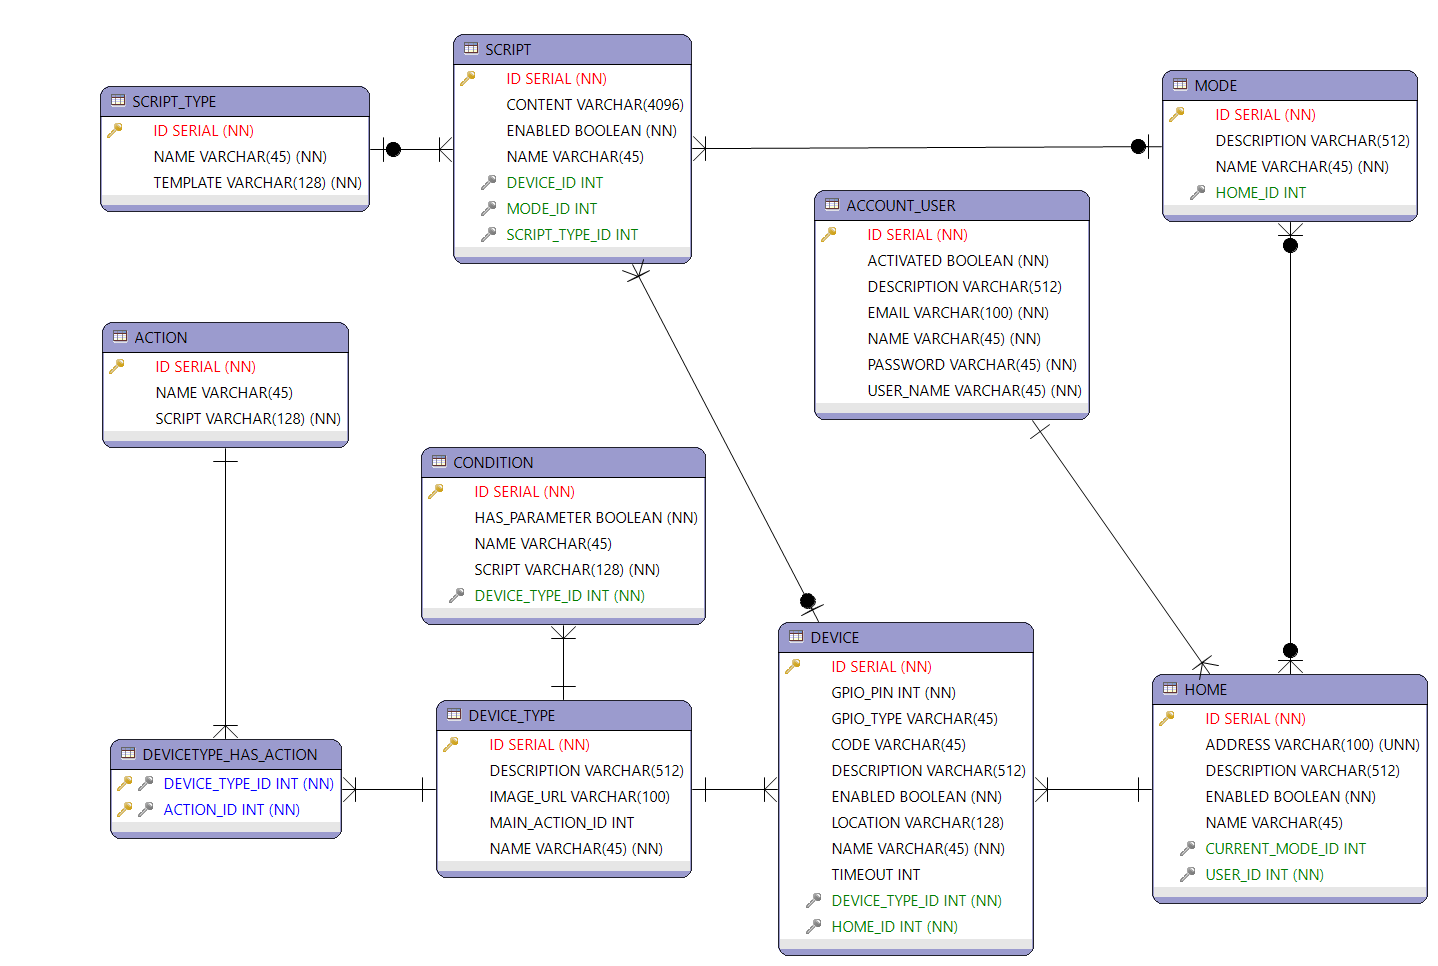
\includegraphics[width=15cm]{3-smart-home-db}
  \caption{Thiết kế database cho ứng dụng}\label{fig:3-smart-home-db}
\end{figure}

Quay lại với yêu cầu được đặt ra từ hệ thống, người dùng có thể có nhiều ngôi nhà. Trong mỗi ngôi nhà sẽ điều khiển nhiều thiết bị khác nhau thuộc nhiều loại khác nhau. Mỗi thiết bị có thể có nhiều kịch bản để tự động hóa chúng. Kịch bản được đặc tả theo dạng điều kiện – hành động, nghĩa là dưới điều kiện nào đó do người dùng quyết định thì sẽ có những hành động tương ứng xảy ra . Những kịch bản sẽ hoặc thuộc dạng đơn giản ( bao gồm 1 điều kiện , 1 hành động ) , hoặc dạng phức tạp mà người dùng có thể tự tạo theo ý muốn riêng của mình. Hơn nữa, với mỗi ngôi nhà có thể có nhiều chế độ quản lý nhưng tại 1 thời điểm chỉ có 1 chế độ được kích hoạt , ví dụ như chế độ đi vắng thì sẽ có những kịch bản riêng , còn với chế độ ở nhà sẽ là bộ kịch bản khác nhằm giúp người dùng tiện lợi trong việc quản lý căn nhà của mình ở nhiều hoàn cảnh khác nhau.

Với cách thiết kế như trên , hệ thống có những đặc điểm

\begin{itemize}[topsep=1mm,itemsep=-0.5mm]
\item Tính thích ứng cao khi có thay đổi yêu cầu
\item Đơn giản trong việc bảo trì và cập nhật ( ví dụ như thêm thiết bị hay loại thiết bị mới )
\vspace{1mm}
\end{itemize}

Chi tiết về chức năng các bảng trong thiết kế được trình bày tại bảng \ref{tab:db-tables}.

\begin{table}
\centering
\caption{Chức năng các bảng trong database}\label{tab:db-tables}
\begin{tabular}{ |l|l|p{10cm}| } 
 \hline
	STT &	Tên bảng &	Chức năng\\ \hline
	1 &	Account\_User &	Thông tin liên quan đến tài khoản người dùng, đã kích hoạt hay chưa, một vài thông tin cá nhân cơ bản\\ \hline
	2 &	Home &	Thông tin liên quan đến nhà , có đang “active” hay không, nhà đang ở chế độ nào\\ \hline
	3 &	Mode &	Thông tin liên quan chế độ được người dùng định nghĩa cho ngôi nhà của mình\\ \hline
	4 &	Device &	Thông tin các thiết bị cho từng nhà  mà hệ thống quản lý như cổng GPIO, có đang “active” không v.v.\\ \hline
	5 &	Device\_Type &	Loại thiết bị hệ thống có thể quản lý như đèn , còi , cảm biến v.v.\\ \hline
	6 &	Script &	Quản lý các thông tin liên quan đến kịch bản, kịch bản người dùng được lưu xuống theo 1 cú pháp định sẵn\\ \hline
	7 &	Script\_Type &	Phân loại kịch bản đơn giản, được cung cấp sẵn hay phức tạp\\ \hline
	8 &	Condition &	Những điều kiện hợp lệ gắn với từng loại thiết bị để sử dụng khi định nghĩa kịch bản\\ \hline
	9 &	Action &	Những hành động hợp lệ gắn với từng loại thiết bị để sử dụng khi định nghĩa kịch bản\\ \hline
	10 &	Device\_Has\_Action &	Mô tả mối quan hệ giữa loại thiết bị và hành động của chúng\\
 \hline
\end{tabular}
\end{table}

\section{Thiết kế và kiến trúc hệ thống back-end}

Hệ thống back-end được hiện thực hoàn toàn dựa trên ngôn ngữ Java và tận dụng sức mạnh từ Spring, một trong những framework được sử dụng nhiều nhất trong Java EE framework. Bằng cách sử dụng framework Spring, việc giao tiếp giữa client và server, cũng như là server với database trở nên dễ dàng hơn. Hơn thế nữa, với đặc trưng của ứng dụng hiện tại là dùng những kịch bản quản lý tự động thiết bị trong nhà, không cần real time(như ứng dụng chat, stream video …) và chỉ gửi yêu cầu tại một số thời điểm, với tần suất nhỏ nên nhóm lựa chọn dùng RESTful web service, xây dựng những API cho client có thể giao tiếp và truy xuất tài nguyên từ server một cách thuận tiện.

\subsection{Spring framework}

Hai khái niệm chính của Spring framework core là "Dependency Injection - DI" và "Aspect Oriented Programming - AOP". Spring framework được sử dụng như là ứng dụng java cơ bản để đạt được kỹ thuật "loose coupling" giữa các components khác nhau bằng cách sử dụng kỹ thuật DI và hỗ trợ việc thực hiện chéo những task vụ như logging, authentication, ... theo kỹ thuật AOP [1][2].

Spring framework cung cấp khá nhiều tính năng khác và số lượng lớn các module cho các mục đích cụ thể, ví dụ như web có Spring MVC, hỗ trợ security có Spring Security, tương tác với datababse có Spring JDBC, và nhiều thứ khác nữa. Ngoài ra, nó còn là một dự án open source với rất nhiều cộng đồng sử dụng, tài liệu tham khảo.

\begin{figure}[h]
  \centering
     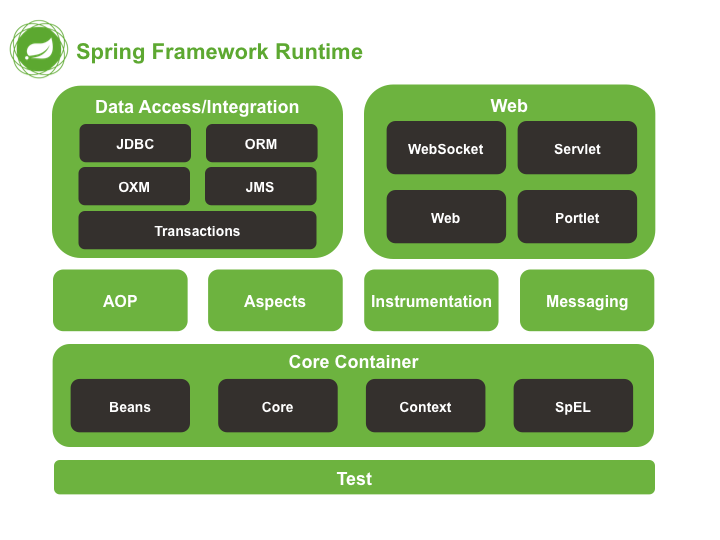
\includegraphics[width=12cm]{3-spring-framework-overview}
  \caption{Tổng quan về Spring Framework}\label{fig:3-spring-framework-overview}
\end{figure}

Một vài tính năng cũng như ưu điểm mà Spring đem đến

\begin{itemize}[topsep=1mm,itemsep=-0.5mm]
\item Dependency Injection hoặc Inversion of Control được sử dụng để giúp các component tách rời, độc lập với nhau. Spring container sẽ giúp gắn kết những components này lại với nhau theo đặc tả business của bạn.
\item Spring MVC framework được sử dụng cho phát triển ứng dụng web rất dễ dàng với việc hỗ trợ rất tốt các tính năng web services, json,... (như RESTful web service framework)
\item Hỗ trợ quản lý transaction, JDBC operations, File uploading, Exception Handling,... rất dễ dàng bằng cách cấu hình được rút gọn, thay vào đó là sử dụng annotation.
\item Làm giảm đi khối lượng code rất nhiều, chẳng hạn như việc khởi tạo đối tượng, open/close các resources,...
\vspace{1mm}
\end{itemize}

\subsection{RESTful Web Service}

Representational State Transfer (REST) định nghĩa các quy tắc kiến trúc để bạn thiết kế Web services chú trọng vào tài nguyên hệ thống, bao gồm các trạng thái tài nguyên được định dạng như thế nào và được chuyển tải qua HTTP thông qua số lượng lớn người dùng và được viết bởi những ngôn ngữ khác nhau. Nếu tính theo số dịch vụ mạng sử dụng, REST đã nổi lên trong vài năm qua như là một mô hình thiết kế dịch vụ chiếm ưu thế[5].

\begin{figure}[h]
  \centering
     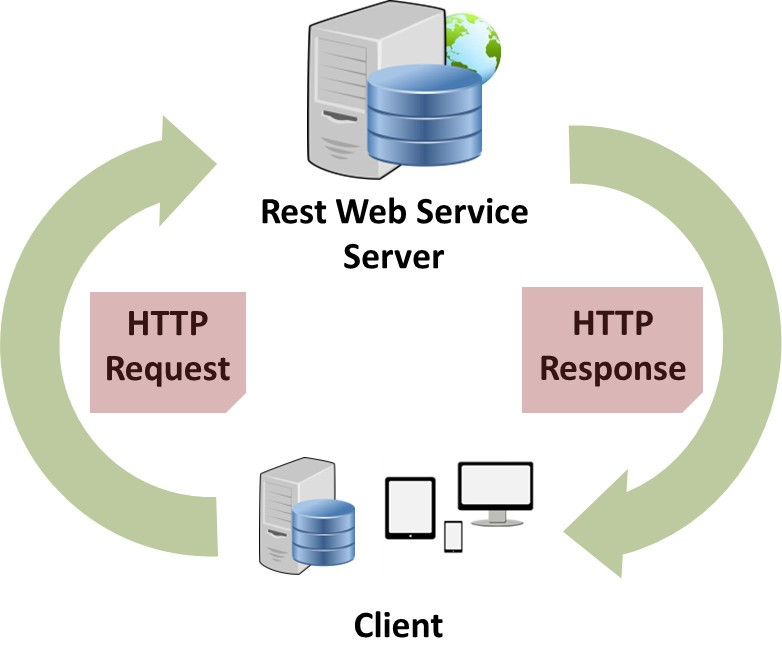
\includegraphics[width=7cm]{3-client-communicate-RESTfulWS}
  \caption{Sơ đồ giao tiếp giữa Client và máy chủ RESTFul Web Service}\label{fig:3-client-communicate-RESTfulWS}
\end{figure}

Những nguyên tắc cơ bản của một RESTFul Web Service:

\begin{itemize}[topsep=1mm,itemsep=-0.5mm]
\item Sử dụng các phương thức HTTP một cách rõ ràng.
\item Phi trạng thái.
\item Hiển thị cấu trúc thư mục như URIs.
\vspace{1mm}
\end{itemize}

\textbf{Sử dụng các phương thức HTTP một cách rõ ràng:} Một đặc tính quan trọng của dịch Web service RESTful là sử dụng một cách rõ ràng các phương thức HTTP theo cách một giao thức được xác định bởi RFC 2616.

REST yêu cầu các nhà phát triển sử dụng phương thức HTTP một cách rõ ràng theo cách tương thích với giao thức chuẩn. Nguyên lý thiết kế REST cơ bản này thiết lập một ánh xạ 1-1 giữa các hành động tạo, đọc, cập nhật và xoá (CRUD) các quá trình vận hành và các phương thức HTTP. Theo cách ánh xạ này thì:

\begin{itemize}[topsep=1mm,itemsep=-0.5mm]
\item Để tạo một tài nguyên trên máy chủ, bạn cần sử dụng phương thức POST.
\item Để truy xuất một tài nguyên, sử dụng GET.
\item Để thay đổi trạng thái một tài nguyên hoặc để cập nhật nó, sử dụng PUT.
\item Để huỷ bỏ hoặc xoá một tài nguyên, sử dụng DELETE.
\vspace{1mm}
\end{itemize}

\textbf{Phi trạng thái:} Một yêu cầu hoàn chỉnh, độc lập không đòi hỏi máy chủ để thu thập được bất kỳ ngữ cảnh hoặc trạng thái của ứng dụng nào trong lúc xử lý yêu cầu. Một ứng dụng (hoặc máy khách) Web service REST chứa ở phần đầu và phần thân trang HTTP của một yêu cầu tất cả các tham số, ngữ cảnh và dữ liệu cần thiết bởi thành phần bên ngoài máy chủ để đưa ra một phản hồi. Phi trạng thái theo nghĩa này nâng cao tính hiệu quả của dịch vụ Web, đơn giản hoá thiết kế và sự thi hành của các thành phần của máy chủ vì khi máy chủ không có trạng thái sẽ huỷ bỏ nhu cầu để đồng bộ hoá các mảng dữ liệu với một ứng dụng bên ngoài.

\textbf{Hiển thị cấu trúc thư mục như URIs:} Các địa chỉ Web service REST nên có tính hiện thực theo nghĩa rằng chúng dễ dàng đối với người dùng. Có thể nghĩ rằng một địa chỉ đường dẫn như là giao diện tự đóng gói mà đòi hỏi ít lý giải hay tham chiếu, nếu có, đối với một nhà phát triển để hiểu nó nhắm đến điểm gì và phân phối tài nguyên liên quan. Cuối cùng, cấu trúc của địa chỉ nên rõ ràng, có thể đoán được và dễ hiểu.
Một cách để đạt được mức độ sử dụng này là xác định cấu trúc thư mục giống URIs. Loại URI này có thứ bậc, có điểm khởi nguồn tại một đường dẫn đơn giản, và có nhánh đi ra là các nhánh phụ thể hiện các vùng chính của dịch vụ. Theo định nghĩa này, một URI không chỉ là một chuỗi bị cắt không giới hạn, mà còn là một cây với các nhánh chính và nhánh dọc nối nhau tại các nút. Ví dụ:

http://www.myservice.org/discussion/topics/{topic}

Các địa chỉ URIs nên giữ nguyên để khi tài nguyên thay đổi hoặc khi tiến hành thay đổi dịch vụ, đường liên kết cũng sẽ giữ nguyên. Việc này cho phép đánh dấu lại vị trí đang đọc. Nó cũng rất quan trọng vì mối liên quan giữa các tài nguyên mà được mã hoá trong các địa chỉ được giữ nguyên độc lập với các mối liên quan đại diện khi chúng được lưu trữ.

Như đã đề cập đến ở phần thiết kế database cho ứng dụng, nhóm quyết định hiện thực trên PostgreSQL. Tận dụng sức mạnh của Spring framework, cùng với sự hỗ trợ của Hibernate framework, những thao tác lưu, truy xuất dữ liệu từ database được thực hiện một cách đơn giản hơn.

\textbf{Hibernate Framework:} Hibernate Framework là một công cụ mã nguồn mở, dung lượng nhỏ (lightweight) và ORM (Object Relational Mapping) giúp đơn giản hóa việc phát triển ứng dụng Java để tương tác với cơ sở dữ liệu. Do Hibernate Framework là một ORM framework cho persistence layer nên khi phát triển ứng dụng, lập trình viên chỉ cần tập trung vào những layer khác(như tầng ứng dụng-business) mà không cần xem xét nhiều về persistence layer, dẫn đến tránh thao tác nhiều với database.

Cấu trúc Hibernate được thể hiện qua hình \ref{fig:3-hibernate-architecture}

\begin{figure}[h]
  \centering
     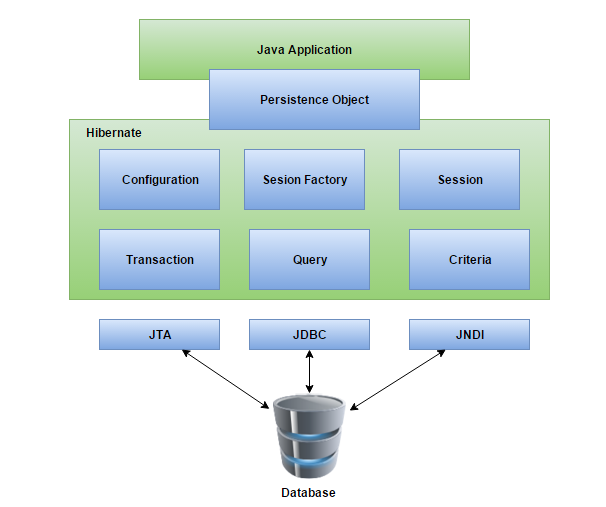
\includegraphics[width=12cm]{3-hibernate-architecture}
  \caption{Cấu trúc Hibernate}\label{fig:3-hibernate-architecture}
\end{figure}

Hibernate sử dụng nhiều API của Java như JDBC, Java Transaction, Java Naming and Directory Interface. JDBC cho  phép bất kỳ cơ sở dữ liệu nào với một trình điều khiển JDBC đều được hỗ trợ bởi Hibernate.

Sau đây là một vài mô tả ngắn gọn về các thành phần trong cấu trúc Hibernate

\begin{itemize}[topsep=1mm,itemsep=-0.5mm]
\item Cấu hình đối tượng(Configuration): nó đại diện cho một tập tin cấu hình, cung cấp thông tin về database muốn kết nối đến. Đây cũng là thành phần tạo ra sự kết nối giữa các Java class và các bảng cơ sở dữ liệu.
\item SessionFactory: đối tượng này được tạo ra trong quá trình ứng dụng khởi động. Mỗi database sử dụng một tập tin cấu hình riêng biệt và chỉ có 1 đối tượng SessionFactory duy nhất. Đối tượng này có thể được truy cập đồng thời bởi nhiều thread nhưng vẫn đảm bảo tính an toàn dữ liệu (thread-safe).
\item Session: đối tượng này được ứng dụng dùng để giao tiếp với database. Các đối tượng Session không nên giữ mở trong thời gian dài vì không an toàn(not thread-safe).
\item Transaction: đối tượng này đại diện cho công việc nhỏ(ví dụ như cập nhật, lưu giá trị). Một session thường bao gồm nhiều transaction.
\item Query: đối tượng truy vấn sử dụng SQL hoặc Hibernate Query Language (HQL) để lấy dữ liệu từ cơ sở dữ liệu.
\item Criteria: kết hợp một hay nhiều tiêu chí để truy xuất một thực thể từ database thỏa mãn
\vspace{1mm}
\end{itemize}

Những lợi ích mà Hibernate đem lại

\begin{itemize}[topsep=1mm,itemsep=-0.5mm]
\item Hibernate Framework là mã nguồn mở theo LGPL licence và dung lượng nhỏ.
\item Đơn giản hóa việc truy nhập, kết nối
\item Hibernate Framework cung cấp các thiết bị để tạo ra các bảng tự động
\item Hỗ trợ hầu hết các loại database management system thông dụng hiện nay
\item Cung cấp cơ chế tự động quản lý cache, cache cấp 1 và cấp 2, giúp tối ưu hóa việc truy xuất dữ liệu.
\vspace{1mm}
\end{itemize}

\subsection{Kiến trúc back-end}

\begin{figure}[h]
  \centering
     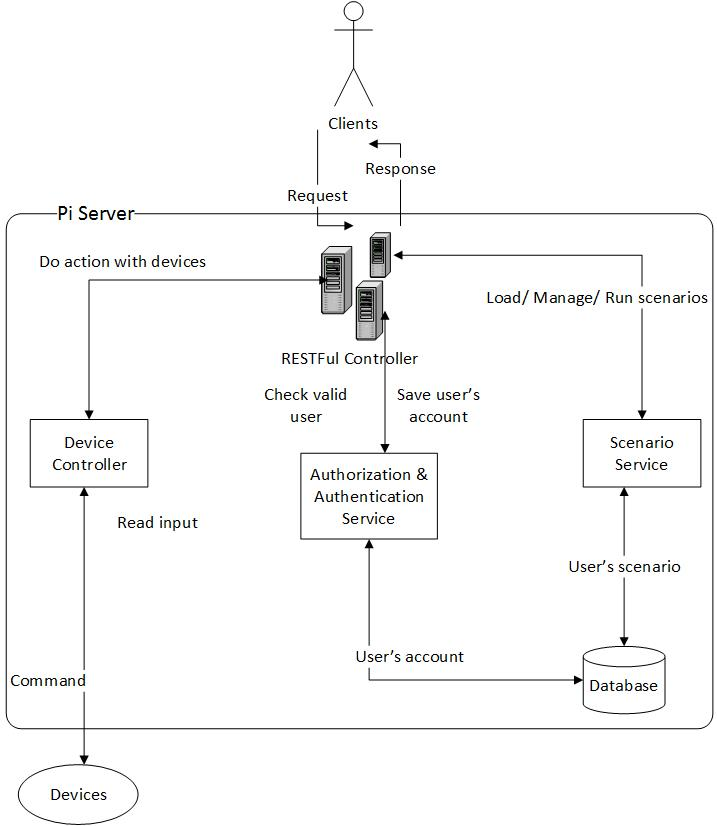
\includegraphics[width=15cm]{3-architecture-back-end}
  \caption{Kiến trúc hệ thống ở back-end}\label{fig:3-architecture-back-end}
\end{figure} 

Hệ thống back-end chia ra làm các module nhỏ

\begin{itemize}[topsep=1mm,itemsep=-0.5mm]
\item Authorization và Authentication service: phục vụ mục đích bảo mật hệ thống, chỉ những người dùng hợp lệ (có tài khoản hợp lệ , có quyền truy xuất với tài nguyên yêu cầu ), quản lý token
\item Scenario Service: quản lý trạng thái các kịch bản ( có đang được kích hoạt chạy hay không ) hay có thay đổi từ nhà hoặc thiết bị ảnh hưởng đến trạng thái kịch bản; quản lý việc thực thi các kịch bản một cách tự động; kiểm tra tính hợp lệ của kịch bản, xác định xem kịch bản có bị mâu thuẫn với chính nó hay với những kịch bản đã tồn tại hay không; cho phép truy xuất , tạo mới , cập nhật kịch bản.
\item Device Service: các kịch bản khi ở trong trạng thái kích hoạt, và thỏa 1 điều kiện định trước do người dùng định nghĩa thì nó sẽ thực thi những hành động tương ứng. Và module này đóng vai trò trung gian trong việc tương tác với thiết bị thật gắn trên Raspberry Pi ở hệ thống back-end , cụ thể là các kịch bản đang chạy.
\vspace{1mm}
\end{itemize}

Chi tiết về hiện thực các module này sẽ nằm trong mục Hiện thực back-end.

%-----------------------------------Device controller---------------------%
\chapter{Module điều khiển thiết bị}
Điều khiển các thiết bị điện trong nhà là một phần không thể thiếu trong hệ thống nhà thông minh. Server cần một bộ điều khiển có thể lấy được dữ liệu từ các cảm biến đặt tại các nơi khác nhau trong nhà, chụp ảnh từ các camera, bật hoặc tắt các thiết bị điện,…Trong chương này, chúng tôi đưa ra các công trình liên quan trong việc sử dụng máy tính siêu nhỏ Raspberry Pi để giải quyết nhiều vấn đề khác nhau trong cuộc sống. Tiếp đến, nhóm trình bày tổng quan thiết kế của module điều khiển thiết bị sử dụng Raspberry Pi và các công nghệ có thể hỗ trợ để hiện thực module.
\newpage
\section{Tổng quan về Raspberry Pi}
Raspberry Pi là một chuỗi các máy tính có kích thước bằng một thẻ tín dụng, được phát triển tại Anh bởi Raspberry Pi Foundation với mục đích giảng dạy khoa học máy tính căn bản.[1] Hình \ref{fig:4-pi3-model-b} mô tả cấu trúc bên ngoài của máy tính Raspberry Pi 3 Model B.

\begin{figure}[h]
  \centering
     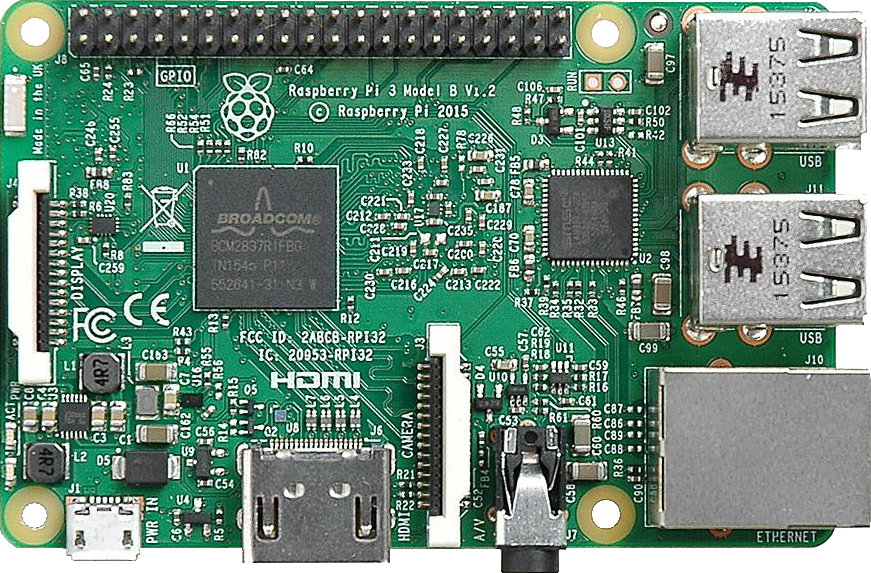
\includegraphics[scale=0.3]{4-pi3-model-b}
  \caption{Máy tính Raspberry Pi 3 Model B}\label{fig:4-pi3-model-b}
\end{figure}

Giá thành của một con Raspberry Pi khá rẻ, phù hợp với túi tiền của tất cả mọi người. Trên thế giới, đã có rất nhiều sản phẩm hữu ích phục vụ cho đời sống và công việc hằng ngày ra đời nhờ sử dụng máy tính Raspberry Pi. Giáo sư Simon Cox và các đồng nghiệp đã lắp ghép 60 con Raspberry Pi bằng các viên gạch Lego để làm thành một chiếc siêu máy tính. Các máy tính Raspberry Pi này hoạt động song song với nhau và cùng giải quyết một vấn đề. Hình \ref{fig:4-Sieu-may-tinh} chụp lại hai trong số 60 con Raspberry Pi làm ra chiếc siêu máy tính [2].

\begin{figure}[h]
  \centering
     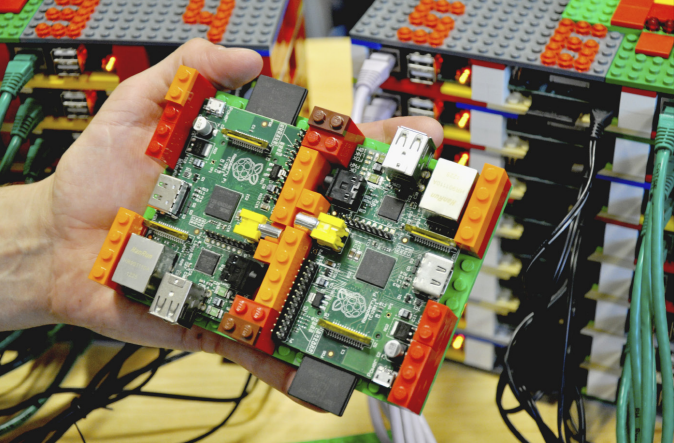
\includegraphics[scale=0.5]{4-Sieu-may-tinh}
  \caption{Siêu máy tính được chế tạo từ các con Raspberry Pi [2]}\label{fig:4-Sieu-may-tinh}
\end{figure}

Một sở thú ở Lodon, Anh cũng sử dụng Raspberry Pi để sáng tạo ra một công cụ gọi là EyesPi, cho phép chụp ảnh các hoạt động thường ngày của các loài động vật trong sở thú. Một người tên Dave Akerman đã cùng những người đồng nghiệp lắp đặt Raspberry Pi trên một khinh khí cầu, sau đó, họ thả bay khinh khí cầu và chụp những bức ảnh về Trái đất khi nhìn từ trên cao [2]. 

\textbf{Các phiên bản:} đã có nhiều thế hệ Raspberry Pi được đưa ra thị trường, phiên bản đầu tiên (Raspberry Pi 1 Model B) được ra mắt vào tháng 2 năm 2012. Từ năm 2012 cho đến nay đã có rất nhiều phiên bản Raspbery Pi ra đời với nhiều cải tiến. Raspberry Pi 3 Model B là phiên bản mới nhất tính đến thời điểm hiện tại, được phát hành vào tháng 2 năm 2016, tích hợp thêm bộ thu phát sóng WiFi và Bluetooth so với phiên bản trước. Đây cũng chính là phiên bản được nhóm lựa chọn sử dụng, thông số kỹ thuật được mô tả tại bảng \ref{tab:pi-3-model-b-specs} [1].

\begin{table}
\centering
\caption{Một vài thông số kỹ thuật của Raspberry Pi 3 Model B}\label{tab:pi-3-model-b-specs}
\begin{tabular}{ |l|l| } 
 \hline
	Vi xử lý		&	ARMv8\\
	Xung nhịp		&	1.2GHz\\
	RAM				&	1 GB SDRAM\\
	Bộ nhớ trong	&	MicroSD\\
	Nguồn điện		&	5V\\
	GPIO			&	40 pin\\
	Video output	&	HDMI\\
	USB 2.0			&	4 cổng\\
	Cổng Ethernet	&	Có hỗ trợ\\
	Wireless		&	802.11n / Bluetooth 4.1\\
 \hline
\end{tabular}
\end{table}

\textbf{Hệ điều hành:} Raspberry Pi đa phần sử dụng một hệ điều hành chuyên dụng là Raspbian. Đây là hệ điều hành mã nguồn mở, được xây dựng dựa trên nền tảng hệ điều hành Debian, được tạo ra bởi một nhóm nhỏ những người hâm mộ Raspberry Pi với mục đích tối ưu hóa cho việc sử dụng phần cứng của Raspberry Pi. Raspbian có khoảng 35000 packages cũng như những phần mềm biên dịch sẵn đính kèm, tiện cho việc cài đặt sử dụng. [1] [7]

Ngoài hệ điều hành Raspbian, Raspberry Pi còn có thể chạy được Windows 10 IoT Core, một hệ điều hành được Microsoft thiết kế để sử dụng riêng cho hệ thống nhúng, và các hệ điều hành có nhân Linux khác như Ubuntu MATE, Xbian, CentOS,…Trong quá trình phát triển ứng dụng, nhóm quyết định cài đặt hệ điều hành Raspbian trên Raspberry Pi vì đây vẫn là hệ điều hành được sử dụng và hỗ trợ nhiều nhất cho Raspberry Pi.

%--------------------------------------------------------------------------%
\section{Điều khiển thiết bị sử dụng GPIO}
Một trong những yếu tố quan trọng của Raspberry Pi là các cổng GPIO (General Purpose Input/Output) được bố trí dọc theo một cạnh của nó. Hình \ref{fig:4-vi-tri-dat-gpio} miêu tả vị trí đặt các cổng GPIO của Raspberry Pi 3 Model B. [6]

\begin{figure}[h]
  \centering
     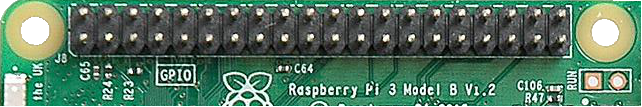
\includegraphics[scale=0.7]{4-vi-tri-dat-gpio}
  \caption{Vị trí đặt các cổng GPIO của Raspberry Pi 3 Model B}\label{fig:4-vi-tri-dat-gpio}
\end{figure}

Mỗi cổng GPIO đều có hai trạng thái là High và Low tương ứng với mức điện áp lần lượt là 3.3V và 0V. Có thể xem các cổng GPIO như một cầu nối giữa Raspberry Pi và thế giới bên ngoài, mỗi cổng cũng có thể là input, cũng có thể là output cho tín hiệu số. Nói một cách đơn giản, mỗi cổng GPIO như một công tắc, người bên ngoài có thể tắt hoặc bật, tức thay đổi trạng thái cổng GPIO, lúc này, GPIO thực hiện chức năng là một cổng input. Các chương trình trên Raspberry Pi cũng có thể thay đổi trạng thái các cổng GPIO, GPIO lúc này thực hiện chức năng là một cổng output, truyền tín hiệu từ các trương trình ra ngoài. [6]

Trong số 40 cổng của Raspberry Pi 3 Model B, có 26 cổng GPIO, 4 cổng nguồn có điện áp luôn luôn là 3.3V hoặc 5V, 8 cổng đất và 2 cổng ID EEPROM được dùng trong các mục đích đặt biệt. Hình \ref{fig:4-vi-tri-phan-bo-gpio} mô tả chi tiết phân bố của các cổng trên Raspberry Pi.

\begin{figure}[h]
  \centering
     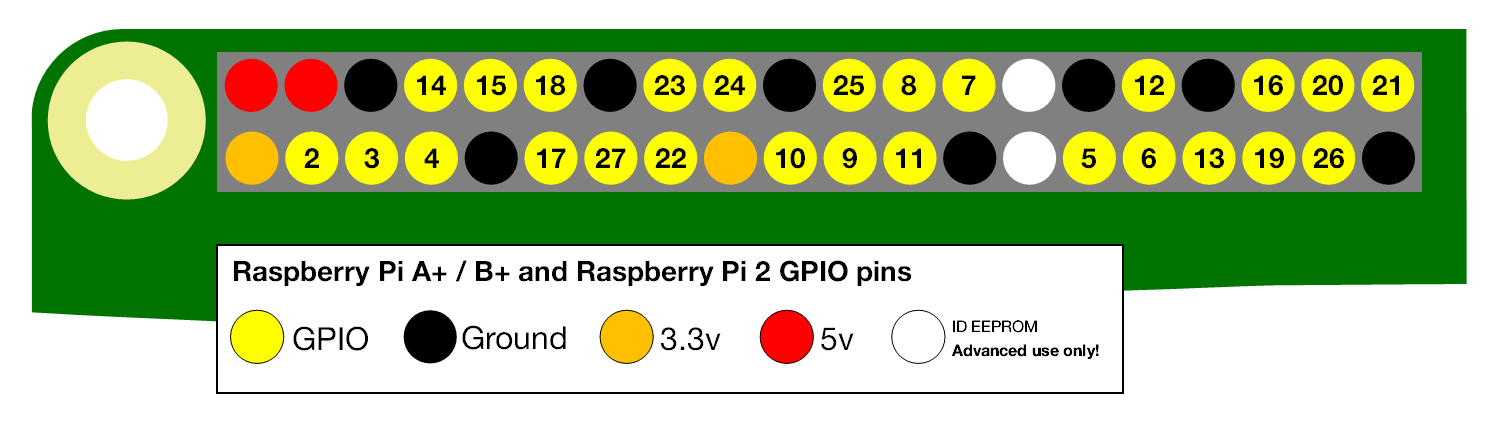
\includegraphics[scale=0.3]{4-vi-tri-phan-bo-gpio}
  \caption{Vị trí phân bố các cổng GPIO}\label{fig:4-vi-tri-phan-bo-gpio}
\end{figure}

Trong số 26 cổng GPIO, một vài cổng có thêm những những chức năng khác ngoài việc thay đổi trạng thái giữa High và Low. Những cổng có thêm những chức năng đặc biệt này được gắn thêm một nhãn tên phía sau như mô tả trong hình …: 

\begin{itemize}[topsep=1mm,itemsep=-0.5mm]
\item UART (Universal Asynchronous Receiver/Transmitter) Serial Bus– GPIO 15, GPIO 16: Giả sử như chúng ta cắm một thiết bị vào mà nó có khả năng hiển thị dữ liệu lên thì khi cắm vào hai chân này, ta có thể đọc được những thông báo từ kernel của Raspberry Pi. Ví dụ như Pi không thể khởi động lên được, ta dùng cách này như một công cụ chẩn đoán lỗi. 

\item I2C (Inter-Integrated Circuit) Bus: cung cấp phương thức giao tiếp giữa nhiều ICs với nhau. Đối với Pi, một IC có thể nhắc đến ngay đó là mạch vi xử lý của nó. I2C bus có thể được truy cập từ GPIO 8 (SDA – Serial Data Line) và GPIO 9 (SCL- Serial Clock). Nó được dùng khá phổ biến để kết nối đến các thiết bị ngoại vi như cảm biến nhiệt độ hay màn hình LCD.

\item SPI (Serial Peripheral Interface) Bus: phục vụ cho in-system programming (ISP). Các GPIO sau hỗ trợ SPI : GPIO 10 ,11, 12, 13, 14.
\vspace{1mm}
\end{itemize}

%---------------------------------Thiết kế chi tiết-------------------------%
\section{Thiết kế chi tiết}

Vai trò chính của module điều khiển thiết bị là nhận yêu cầu từ server gửi đến và thực hiện đúng hành động mà server mong muốn. Để hiện thực chức năng này, các thiết bị được gắn trực tiếp vào một máy tính siêu nhỏ gọi là Raspberry Pi, mỗi thiết bị được điều khiển thông qua các chân cắm gọi là GPIO nằm dọc một cạnh của Raspberry Pi. Hình \ref{fig:4-module-dieu-khien-overview} mô tả sự tương tác giữa server, module điều khiển thiết bị và Raspberry Pi.

\begin{figure}[h]
  \centering
     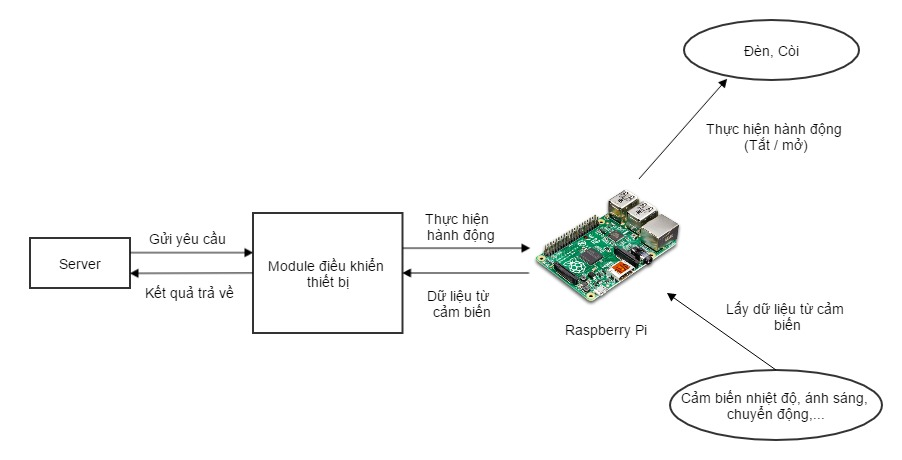
\includegraphics[scale=0.5]{4-module-dieu-khien-overview}
  \caption{Sơ đồ tổng quan của module điều khiển thiết bị}\label{fig:4-module-dieu-khien-overview}
\end{figure}

Ví dụ, khi server muốn thực hiện hành động tắt đèn phòng khách, server sẽ gửi yêu cầu đến module điều khiển thiết bị kèm theo thông tin về thiết bị mà server cần điều khiển, trong trường hợp này là thông tin về chiếc đèn phòng khách. Trong những thông tin mà server gửi đến module điều khiển thiết bị thì số thứ tự cổng GPIO mà thiết bị này kết nối vào là thông tin quan trọng. Vì mỗi thiết bị sẽ được điều khiển bởi một GPIO, module điều khiển thiết bị cần biết chính xác chiếc đèn phòng khách được điều khiển bởi GPIO nào để thực hiện đúng hành động và đúng mục tiêu.

Module điều khiển thiết bị được thiết kế gồm hai phần chính, được trình bày chi tiết tại hình \ref{fig:4-module-dieu-khien-detail}, bao gồm: bộ điều khiển tổng quát (General controller) và bộ cung cấp cổng GPIO (GPIO provider).

\begin{figure}[h]
  \centering
     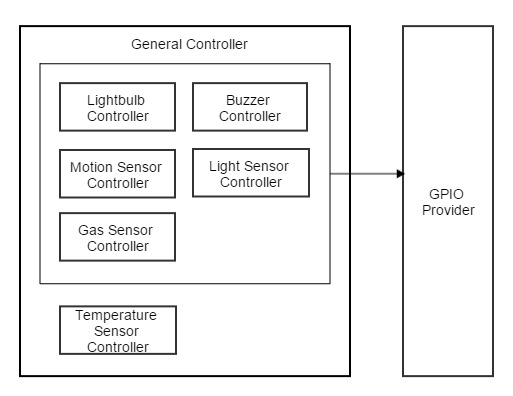
\includegraphics[scale=0.5]{4-module-dieu-khien-detail}
  \caption{Thiết kế chi tiết module điều khiển thiết bị}\label{fig:4-module-dieu-khien-detail}
\end{figure}

\textbf{Bộ điều khiển tổng quát (General controller):} vai trò của bộ điều khiển tổng quát là nhận tất cả yêu cầu được gửi đến tử server và xử lý tất cả yêu cầu này, xác định xem đây là yêu cầu dành cho loại thiết bị nào và sử dụng đúng bộ điều khiển dành cho loại thiết bị đó. Trong bộ điều khiển tổng quát có chứa nhiều bộ điều khiển con dành cho từng loại thiết bị, tùy vào yêu cầu của server mà bộ điều khiển tổng quát sẽ quyết định sử dụng bộ điều khiển con nào. 

Bộ điều khiển camera (Camera controller) được dùng để chụp ảnh với camera chuyên dụng của Raspberry Pi. Với sự hỗ trợ của thư viện JRPiCam, bộ điều khiển camera có thể dễ dàng điều chỉnh các thông số từ chất lượng ảnh cho đến độ sáng, độ nét và độ tương phản. Các bộ điều khiển cảm biến (Gas sensor controller, Light sensor controller,…) lấy dữ liệu từ các cảm biến thông qua các cổng GPIO. Dữ liệu trả về có thể thuộc dạng số thực, như nhiệt độ hoặc dạng đúng/sai như có gas hay không?, trời sáng hay không?, ...

Hai bộ điều khiển còn lại là bộ điều khiển đèn (Lightbulb controller) và bộ điều khiển còi (Buzzer controller) có vai trò như một công tắt đóng/mở. Mỗi thiết bị đèn hoặc còi sẽ được điều khiển bởi một cổng GPIO. Như đã trình bày, mỗi cổng GPIO đều có hai trạng thái là Low và Hight, tùy thuộc vào người thiết kế hệ thống mà từng trạng thái của GPIO sẽ tương ứng với bật hay tắt thiết bị. Trong dự dán của mình, nhóm sử dụng trạng thái Low là bật và trạng thái Hight là tắt.

\textbf{Bộ cung cấp GPIO (GPIO provider):} bộ cung cấp GPIO có vai trò khai báo và cung cấp chính xác loại cổng mà bộ điều khiển thiết bị cần. Với các bộ điều khiển thiết bị dành cho cảm biến, bộ cung cấp GPIO cần khởi tạo cổng nhập (input pin) có chức năng nhận dữ liệu từ cảm biến. Đối với bộ điều khiển thiết bị cho đèn hoặc còi, bộ cung cấp GPIO cần khởi tạo cổng xuất (output pin) sử dụng cho việc điều khiển trạng thái bật/tắt.
%------------------------------------------------------------------------%

%--------------------------Công nghệ hỗ trợ---------------------------%
\section{Công nghệ hỗ trợ}
Có rất nhiều thư viện được viết bằng nhiều ngôn ngữ khác nhau hỗ trợ việc điều khiển các cổng GPIO của Raspberry Pi. Bên dưới là một vài công nghệ đang được sử dụng phổ biến hiện nay.

\textbf{Thư viện Pi4J:} Pi4J là một thư viện được viết bằng ngôn ngữ Java với mục đích cung cấp các API (Application Programming Interface) cho người lập trình có thể điều khiển dễ dàng các cổng GPIO mà không cần quan tâm đến cấu trúc bên dưới của Raspberry Pi.

\textbf{Thư viện WiringPi:} cũng là một thư viện được sử dụng để điều khiển các cổng GPIO, thư viện WiringPi được viết bằng ngôn ngữ C, là một thư viện hiệu quả đối với những chương trình viết bằng C hoặc C++. Tuy nhiên, đã có nhiều lập trình viên tạo thêm những phiên bản phù hợp với những loại ngôn ngữ khác như Java, Python, Ruby,…

\textbf{Thư viện RPi.GPIO:} là một thư viện được viết bằng ngôn ngữ Python, RPi.GPIO được tạo ra với mục đích cung cấp những API cần thiết cho người lập trình Python có thể điều khiển các cổng GPIO của Raspberry Pi một cách dễ dàng

\textbf{Thư viện JRPiCam:} được tạo ra với mục đích cung cấp các API dành cho việc sử dụng camera chuyên dụng của Raspberry Pi, giúp người lập trình dễ dàng hơn trong việc sử dụng và cấu hình camera. JRPiCam được viết bằng ngôn ngữ Java, mã nguồn được công bố công khai tại GitHub.

\textbf{Thư viện Picamera:} giống như JRPiCam, Picamera cung cấp các API sử dụng cho việc điều khiển và cấu hình camera của Raspberry. Tuy nhiên, Picamera được viết bằng ngôn ngữ Python.

Sau khi tìm hiểu các công nghệ có thể hỗ trợ, chúng tôi quyết định chọn thư viện Pi4J sử dụng cho việc lấy dữ liệu và điều khiển trạng thái các cổng GPIO, thư viện JRPiCam sẽ được dùng để hiện thực bộ điều khiển camera. Lý do nhóm quyết định lựa chọn hai thư viện này vì đây đều là những thư viện mã nguồn mở, được công bố công khai tại GitHub. Vì vậy, nhóm có thể tùy chỉnh lại mã nguồn nếu cần thiết để tăng hiệu suất của hệ thống. Bên cạnh đó, phương pháp lập trình nhóm hướng đến là lập trình hướng đối tượng, nên chúng tôi ưu tiên sử dụng những thư viện được viết bằng ngôn ngữ Java.

Với thiết kế của module điều khiển thiết bị đã được nêu ở những phần trên, tuy không thể điều khiển được tất cả các thiết bị có trong nhà, nhưng đủ để nhóm có thể tạo ra một mô hình thí nghiệm với đầy đủ các thiết bị cần thiết như các cảm biến, đèn, còi và camera. Server được cung cấp đầy đủ các API để điều khiển tất cả các thiết bị hiện có phục vụ cho các mục đích khác nhau như bật/tắt đèn hoặc còi, lấy nhiệt độ, kiểm tra khí gas,…Chi tiết hiện thực module điều khiển thiết bị sẽ được trình bày tại chương …

%------------------------------------------------------------------------%

%-----------------------------------Mobile app-----------------------------%
\chapter{Ứng dụng di động}

%--------------------------------Các chức năng của ứng dụng--------------%
\newpage
\section{Các chức năng của ứng dụng}
Ứng dụng di động nhà thông minh được thiết kế để hỗ trợ người dùng dễ dàng:
\begin{itemize}[topsep=1mm,itemsep=-0.5mm]
\item Đăng ký và đăng nhập vào hệ thống
\item Quản lý các ngôi nhà được lắp đặt hệ thống
\item Quản lý các Chế độ người dùng tự tạo của ngôi nhà
\item Quản lý các thiết bị hệ thống hỗ trợ được lắp đặt vào nhà
\item Quản lý các Kịch bản định sẵn của từng thiết bị
\item Quản lý các Kịch bản người dùng tự tạo của ngôi nhà
\vspace{1mm}
\end{itemize}

-------------------------------------------------------------------------%
\section{Kiến trúc tổng quát}
Hình \ref{fig:5-UI-Flow} mô tả sơ đồ luồng Giao diện của ứng dụng di động.

\begin{figure}[h]
  \centering
     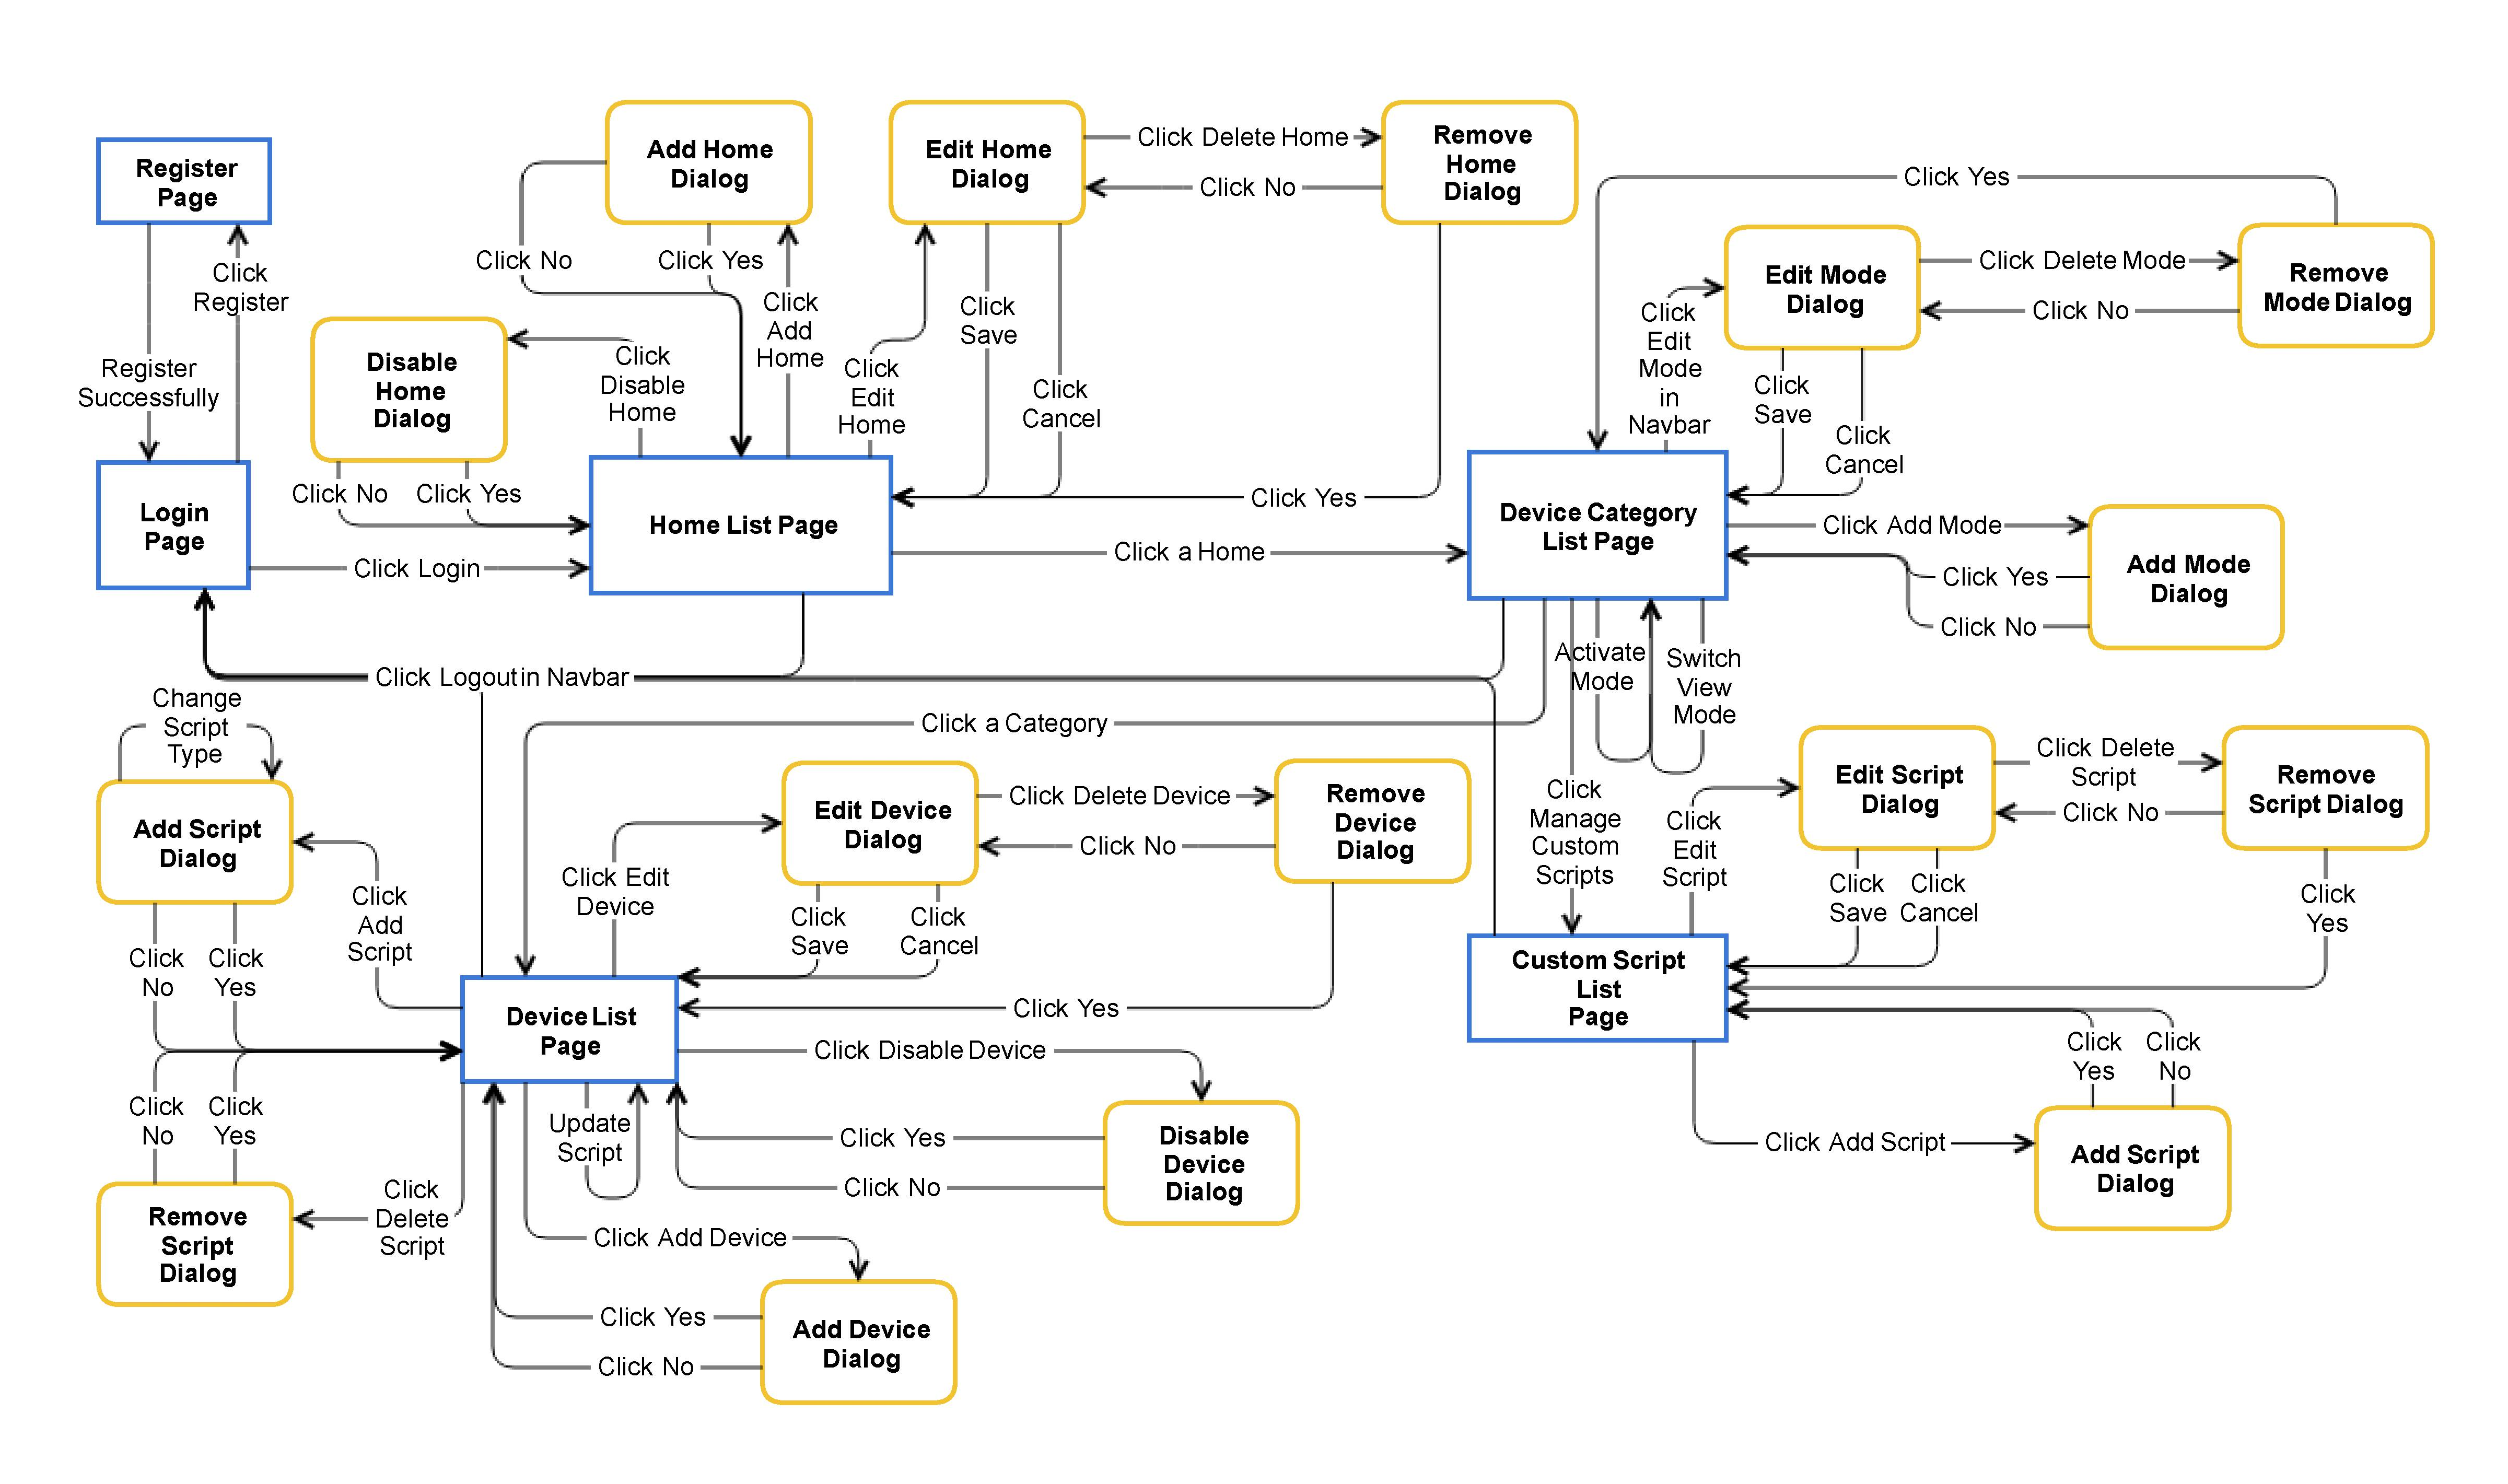
\includegraphics[width=16cm]{5-UI-Flow}
  \caption{Sơ đồ luồng Giao diện của ứng dụng di động}\label{fig:5-UI-Flow}
\end{figure}

Ứng dụng có kiến trúc bao gồm 6 Giao diện (Page) chính là Giao diện Đăng nhập, Giao diện Đăng ký, Giao diện Danh sách các ngôi nhà, Giao diện Danh sách các kiểu thiết bị, Giao diện Danh sách các thiết bị và Giao diện Danh sách các kịch bản tự tạo. Trong mỗi Giao diện chính có các Bảng hộp thoại (Dialog) hỗ trợ người dùng thực hiện các chức năng của ứng dụng.

\textbf{Giao diện Đăng ký (Register Page):} Giao diện cho phép người dùng đăng ký tài khoản hệ thống với các thông tin là Tên đầy đủ, Tên đăng nhập, Mật khẩu, Xác nhận mật khẩu và địa chỉ Email. Sau khi người dùng nhập đầy đủ các thông tin và gửi lên hệ thống, một Email sẽ được gửi tới địa chỉ Email của người dùng để xác nhận các thông tin đăng ký. Giao diện này không có Bảng hộp thoại nào. Từ Giao diện này, người dùng có thể đến Giao diện đăng nhập sau khi đã gửi thông tin đăng ký.

\textbf{Giao diện Đăng nhập (Login Page):} Giao diện cho phép người dùng đăng nhập vào hệ thống với tên tài khoản và mật khẩu mà người dùng đã đăng ký. Giao diện này không có Bảng hộp thoại nào. Từ giao diện này người dùng có thể đi đến Giao diện đăng ký bằng cách nhấn nút Đăng ký (Register) hoặc đến Giao diện Danh sách các ngôi nhà sau khi đã đăng nhập thành công.

\textbf{Giao diện Danh sách các ngôi nhà (Home List Page):} Danh sách tên các ngôi nhà được lắp đặt hệ thống của người dùng được thể hiện ở Giao diện này. Với mỗi ngôi nhà, khi người dùng nhấn nút chỉnh sửa, Bảng hộp thoại Chỉnh sửa ngôi nhà sẽ hiện ra, tại đây người dùng có thể xem đầy đủ cũng như cập nhật lại thông tin của ngôi nhà, bao gồm Tên, Địa chỉ và Mô tả. Để xóa một ngôi nhà, người dùng có thể nhấn nút Xóa (Remove Home) tại Bảng hộp thoại này, một Bảng hộp thoại khác hiện lên yêu cầu người dùng xác nhận thao tác Xóa. Để thêm mới một ngôi nhà, người dùng có thể nhấn nút Thêm mới (Add Home) tại Giao diện chính để mở Bảng hộp thoại Thêm mới yêu cầu người dùng nhập đầy đủ các thông tin về nhà mới. Ngoài ra, người dùng còn có thể dừng hoạt động của hệ thống hoặc cho phép hệ thống hoạt động trở lại tại mỗi ngôi nhà thông qua việc nhấn nút Tắt/Mở (Disable/Enable). Từ giao diện này, khi nhấn Đăng xuất (Logout) từ thanh công cụ, người dùng sẽ về Giao diện Đăng nhập hoặc khi nhấn vào một ngôi nhà, người dùng sẽ tới Giao diện Danh sách các kiểu thiết bị.

\textbf{Giao diện Danh sách các kiểu thiết bị (Device Category List Page):} Danh sách tên các kiểu thiết bị và Danh sách tên các chế độ thuộc ngôi nhà được chọn sẽ được thể hiện ở Giao diện này. Tại đây, người dùng có thể chuyển đổi Chế độ (Mode) thông qua hộp trình đơn thả xuống (Dropdown box) hoặc kích hoạt (Activate) một Chế độ bất kì bằng cách nhấn vào tên Chế độ đó tại thanh công cụ. Để chỉnh sửa thông tin hoặc xóa một Chế độ nào đó, người dùng nhấn vào nút chỉnh sửa cạnh tên Chế độ đó tại thanh công cụ. Để thêm mới một Chế độ, người dùng có thể nhấn nút Thêm mới (Add Mode) tại giao diện chính để mở Bảng hộp thoại Thêm mới yêu cầu người dùng nhập đầy đủ các thông tin về Chế độ mới. Từ giao diện này, khi nhấn Đăng xuất (Logout) từ thanh công cụ, người dùng sẽ về Giao diện Đăng nhập, khi nhấn vào một kiểu thiết bị, người dùng sẽ tới Giao diện Danh sách các thiết bị hoặc khi nhấn vào nút Quản lý Kịch bản tự tạo (Manage Custom Scripts), người dùng sẽ tới Giao diện Danh sách các Kịch bản tự tạo.

\textbf{Giao diện Danh sách các thiết bị (Device List Page):} Danh sách tên, chân GPIO các thiết bị thuộc kiểu thiết bị được chọn cũng như Danh sách các Kịch bản định sẵn thuộc Chế độ được chọn của từng thiết bị được thể hiện ở Giao diện này. Với mỗi thiết bị, khi người dùng nhấn nút chỉnh sửa, Bảng hộp thoại Chỉnh sửa thiết bị sẽ hiện ra, tại đây người dùng có thể xem đầy đủ cũng như cập nhật lại thông tin của thiết bị, bao gồm Tên, Mô tả và Vị trí. Để xóa một thiết bị, người dùng có thể nhấn nút Xóa (Remove Device) tại Bảng hộp thoại này, một Bảng hộp thoại khác hiện lên yêu cầu người dùng xác nhận thao tác Xóa. Để thêm mới một thiết bị, người dùng có thể nhấn nút Thêm mới (Add Device) tại Giao diện chính để mở Bảng hộp thoại Thêm mới yêu cầu người dùng nhập đầy đủ các thông tin về thiết bị mới. Danh sách các Kịch bản thuộc một thiết bị sẽ được thể hiện khi người dùng nhấn vào thiết bị đó, người dùng có thể Xóa Kịch bản bằng cách nhấn nút Xóa ở đầu mỗi Kịch bản hoặc cập nhật lại thông tin Kịch bản như Điều kiện, Hành động hay Thời gian bắt đầu, Thời gian kết thúc thông qua các hộp trình đơn thả xuống. Ngoài ra để thêm mới một Kịch bản, người dùng có thể nhấn nút Thêm mới Kịch bản (Add Script), Bảng hộp thoại Thêm mới Kịch bản hiện ra, người dùng cần chọn Loại Kịch bản muốn thêm và xác định nội dung cho kịch bản đó. Từ giao diện này, khi nhấn Đăng xuất (Logout) từ thanh công cụ, người dùng sẽ về Giao diện Đăng nhập hoặc khi nhấn vào biểu tượng Ngôi nhà (Home) trên thanh công cụ, người dùng sẽ quay lại Giao diện Danh sách các kiểu thiết bị.

\textbf{Giao diện Danh sách các Kịch bản tự tạo (Custom Script List Page):} Danh sách tên các Kịch bản người dùng tự tạo thuộc Chế độ được chọn sẽ được thể hiện ở Giao diện này. Với mỗi Kịch bản tự tạo, khi người dùng nhấn nút chỉnh sửa, Bảng hộp thoại Chỉnh sửa Kịch bản tự tạo sẽ hiện ra, tại đây người dùng có thể xem cũng như cập nhật lại nội dung và tên của kịch bản. Để thêm mới một Kịch bản tự tạo, người dùng có thể nhấn nút Thêm mới Kịch bản tự tạo (Add Custom Script), Bảng hộp thoại Thêm mới Kịch bản tự tạo hiện ra yêu cầu người dùng xác định tên và nội dung cho kịch bản mới. Từ giao diện này, khi nhấn Đăng xuất (Logout) từ thanh công cụ, người dùng sẽ về Giao diện Đăng nhập hoặc khi nhấn vào biểu tượng Ngôi nhà (Home) trên thanh công cụ, người dùng sẽ quay lại Giao diện Danh sách các kiểu thiết bị.

Với cách thiết kế như trên, kiến trúc ứng dụng di động cung cấp một giao diện tương đối đơn giản nhưng vẫn đáp ứng được các nhu cầu cơ bản về việc quản lý các ngôi nhà, thiết bị, chế độ và các kịch bản điều khiển thiết bị của người dùng.

%-----------------------------------Hiện thực và đánh giá------------------%
\chapter{Hiện thực và đánh giá}
\newpage
\section{Hiện thực server back-end}

\subsection{RESTFul Web Service - Cách thức giao tiếp giữa client và server}

Như đã đề cập ở phần Thiết kế back-end, nhóm đã chọn dùng RESTful web service làm cách giao tiếp chính giữa client và server. Một tiện ích khi sử dụng Spring framework đó là nó có hỗ trợ sẵn annotation @RestController, đơn giản hóa việc tạo ra các RESTful web services.

\begin{figure}[h]
  \centering
     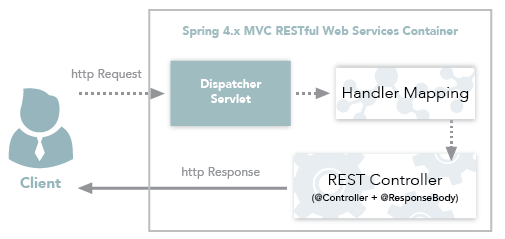
\includegraphics[width=12cm]{6-spring-RESTfulWS-workflow}
  \caption{Spring MVC RESTful Web services workflow}\label{fig:6-spring-RESTfulWS-workflow}
\end{figure} 

Hình \ref{fig:6-spring-RESTfulWS-workflow} diễn tả luồng thực thi của Spring MVC REST, bao gồm các bước sau:

\begin{itemize}[topsep=1mm,itemsep=-0.5mm]
\item Client gửi yêu cầu đến web service theo như một định dạng URI nào đó có sẵn và hợp lệ
\item Yêu cầu đi qua Servlet Dispacher đầu tiên và nó sẽ tìm ra 1 controller phù hợp nhất để xử lý yêu cầu đó
\item Yêu cầu sau khi được xử lý bởi controller sẽ được gửi trả về client dưới định dạng JSON[3].
\vspace{1mm}
\end{itemize}

Danh sách API có thể được tham khảo thêm ở mục Phụ lục

\subsection{Cách thức giao tiếp với database}
Như đã đề cập ở mục thiết kế hệ thống back-end bên trên, nhóm sử dụng Hibernate framework để hỗ trợ cho các thao tác liên quan đến database. Hibernate cung cấp sẵn các hàm giúp truy xuất, lưu, cập nhật, xóa thực thể liên quan. Dựa trên đó, nhóm đã thiết kế ra 1 tầng thao tác dữ liệu (DAO) có cấu trúc như sau

%\begin{figure}[h]
%  \centering
%    \includesvg[width=12cm]{6-DAO-structure}
%  \caption{ Tổ chức của tầng truy xuất dữ liệu(DAO)}\label{fig:6-DAO-structure}
%\end{figure}

Thiết kế này giúp tăng khả năng tái sử dụng (reuse), cũng như việc quản lý, bảo trì, mở rộng hệ thống được dễ dàng hơn trong tương lai. Ý tưởng cơ bản là có 1 class BaseDao, được hiện thực đầy đủ các hàm save(), update(), delete(), ... còn các thực thể khác (như Home, User, Mode, Device, Script) thì thừa kế class BaseDao này và hiện thực thêm một số phương thức khác tùy theo nhu cầu.

Nếu những thao tác với database gây ra lỗi, dữ liệu sẽ được rollback ngay thời điểm đó(ví dụ như vi phạm constraint, khóa ngoại-foreign key, … ), nhằm đảm bảo tính nhất quán của dữ liệu.

\subsection{giới thiệu về kịch bản(scenario)}

Kịch bản là một bản phác thảo, diễn tả những hành vi mình mong muốn thiết bị trong nhà sẽ tự động thực hiện trong hoàn cảnh nhất định hay điều kiện nào đó thỏa mãn. 

\textbf{Kịch bản người dùng:} Kịch bản người dùng sử dụng ngôn ngữ tự nhiên để đặc tả. Lấy ví dụ như “Trong khoảng thời gian từ 18h tối đến 22h tối thì bật đèn ở hành lang lên”. Vế đầu “trong khoảng thời gian từ 18h tối đến 22h tối” đặc tả điều kiện, vế sau “bật đèn hành lang” nêu ra hành động mong muốn khi mà điều kiện trên thỏa mãn.

\textbf{Kịch bản hệ thống:} Kịch bản hệ thống được đặc tả bởi văn phạm riêng(sẽ được giới thiệu ở mục 3.5), nhằm giúp hệ thống có khả năng “đọc”, “hiểu” kịch bản của người dùng.

\subsection{Văn phạm(Grammar) dùng tạo ra kịch bản hệ thống}

Kịch bản của người dùng thường được đặc tả bởi ngôn ngữ tự nhiên. Với hệ thống hiện tại của nhóm, tính năng xử lý ngôn ngữ tự nhiên không được hỗ trợ, do đó vấn đề cấp thiết đặt ra đầu tiên và cũng không kém phần quan trọng, chính là đặc tả văn phạm cho kịch bản. Đặc tả văn phạm kịch bản nhằm giúp hệ thống phân định được kịch bản nào là hợp lệ và kịch bản nào không hợp lệ. Hơn thế nữa, văn phạm giúp hệ thống có thể “đọc”, “hiểu” và xử lý kịch bản. Tuy nhiên, công việc khó khăn là làm sao văn phạm đặc tả chính xác được kịch bản mà vẫn giữ đúng ý nghĩa của nó. Sau thời gian nghiên cứu, nhóm quyết định chọn BNF (Backus-Naur form), gồm những kí hiệu toán học để đặc tả văn phạm cho ngôn ngữ phi ngữ cảnh, thường dùng để xây dựng cú pháp các ngôn ngữ trong ngành máy tính, ví dụ như ngôn ngữ lập trình, tập lệnh... áp dụng vào việc xây dựng văn phạm kịch bản hệ thống.

Dưới đây là văn phạm mà nhóm dùng để mô tả những kịch bản hệ thống, bao gồm từ khóa (đặt trong cặp ngoặc kép), kí hiệu, phép toán, cấu trúc (đặt trong <>):

\begin{table}[h]
\centering
\caption{Cấu trúc văn phạm}\label{tab:grammars}
\begin{tabular}[t]{ lll } 
	<Scenario>	&	::= & 
	\begin{tabular}[t]{l}
	[“ <ControlBlock> “] | “[“ <Scenario> “,”  <ControlBlock> “]” \\ 
	| “[“ <SimpleAction> “]” | “[“ <Scenario>  “,”  <SimpleAction> “]”
	\end{tabular}\\
	
	<ControlBlock> 	&	::=	&
	\begin{tabular}[t]{l}
	“[‘If’ ,“  <Condition>  “,”  <Action> “]” \\
	| “[‘If’,” <Condition> “,” <Action> “,” <Action> “]” \\
	| <FromToBlock>
	\end{tabular}\\
	
	<Condition>  & ::= &
	\begin{tabular}[t]{l}
	“[“ <DeviceName> “,”  <RelationalOperator> “,”  <Value> “]”
	\end{tabular}\\
	
	<Action> & ::= &
	\begin{tabular}[t]{l}
	<Scenario>
	\end{tabular}\\
	
	<FromToBlock> &	::= &
	\begin{tabular}[t]{l}
	“[‘FromTo’,”  Time “,” Time “,”  <Action>  “]” 
	\end{tabular}\\
	
	<RelationalOperator> &	::= &
	\begin{tabular}[t]{l}
	<Equal> | <NotEqual> | < GreaterThan > \\
	| <GreaterThanEqual> | <LessThan> | <LessThanEqual> 
	\end{tabular}\\
	
	<SimpleAction> & ::= &
	\begin{tabular}[t]{l}
	“[‘TurnOn’,”  <DeviceName> “]“\\
	| “[‘TurnOff’,”  <DeviceName> “]”\\
	| “[‘Toggle’,” <DeviceName> “]”\\
	| “[‘TakePicture’,”  <DeviceName> “]”
	\end{tabular}\\
	
	<DeviceName> & ::= & String \\
	
	<Value> & ::= &	Long | Boolean \\
	
	<Equal> & ::= &	“=” \\
	
	<NotEqual> 	& ::= & “!=” \\
	
	<GreaterThan> &	::= & “>” \\
	
	<GreaterThanEqual> & ::= & “>=” \\
	
	<LessThan> 	& ::= & “<” \\
	
	<LessThanEqual>	& ::= & “<=”
	
	
\end{tabular}
\end{table}

\newpage
\section{Xây dựng module điều khiển thiết bị}
\subsection{Lắp đặt thiết bị}
Để Raspberry Pi có thể điều khiển được các thiết bị thông qua các chân GPIO, đầu tiên, chúng ta phải lắp đặt đúng cách thiết bị đó vào Raspberry Pi. Nhằm mục đích đảm bảo an toàn và thuận tiện trong việc tiến hành thí nghiệm, chúng tôi ưu tiên sử dụng những thiết bị điện yêu cầu hiệu điện thế thấp (từ 5V trở xuống).

\textbf{Lắp đặt đèn:} Đèn được sử dụng trong thí nghiệm là loại đèn led bốn chân tích cực mức cao. Một chân của đèn led sẽ luôn luôn được nối vào cổng Ground của Raspberry Pi, một chân còn lại (chân red, green hoặc blue) sẽ được nối vào một GPIO. Khi GPIO ở trạng thái High, tức mức điện áp đưa vào là 3.3V, đèn led sẽ sáng, ngược lại, đèn sẽ tắt. Hình \ref{fig:6-rgb-led} trình bày thông tin các chân của đèn led. Ngoài led ba màu, nhóm còn sử dụng thêm loại led chỉ có hai chân được sử dụng rộng rãi, cách lắp đặt tương tự như đèn led bốn chân.

\begin{figure}[h]
  \centering
     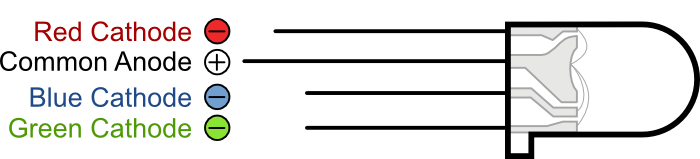
\includegraphics[scale=1.0]{6-rgb-led}
  \caption{Thông tin các chân của đèn led [1]}\label{fig:6-rgb-led}
\end{figure}

\textbf{Lắp đặt còi:} Còi là một thiết bị không thể thiếu trong các căn nhà thông minh, mục đích chủ yếu là để cảnh báo chủ nhà đang có nguy hiểm xảy ra. Loại còi được nhóm sử dụng trong mô hình nhà thông minh gồm có ba chân: VCC, GND và Signal. Hình \ref{fig:6-buzzer} mô tả vị trí các chân nằm trên module còi. Hai chân VCC và GND sẽ lần lượt được gắn vào hai cổng luôn luôn có hiệu điện thế lần lượt là 3.3V và 0V, chân Signal sẽ được gắn vào một cổng GPIO có nhiện vụ điều khiển. Loại còi mà nhóm sử dụng thuộc loại tích cực mức thấp nên còi sẽ bắt đầu hú khi trạng thái của GPIO điều khiển là Low.

\begin{figure}[h]
  \centering
     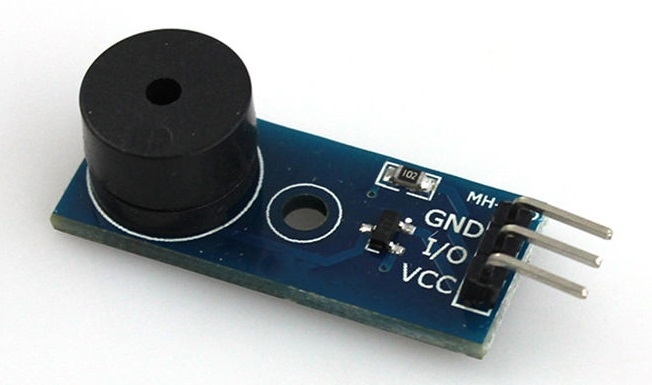
\includegraphics[scale=0.3]{6-buzzer}
  \caption{Module còi gồm 3 chân: VCC, GND và Signal (nằm giữa) [2]}\label{fig:6-buzzer}
\end{figure}

\textbf{Lắp đặt camera:} Nhóm sử dụng camera chuyên dụng của Rasperry Pi để dùng cho việc chụp ảnh. Cách lắp đặt camera cũng khá đơn giản, trên Raspberry Pi có một cổng cắm camera nằm giữa cổng HDMI và cổng Ethernet. Hình \ref{fig:6-camera} mô tả vị trí cổng cắm camera. Chỉ cần gắn dây camera vào đúng cổng trên Raspberry Pi là việc lắp đặt hoàn tất.

\begin{figure}[h]
  \centering
     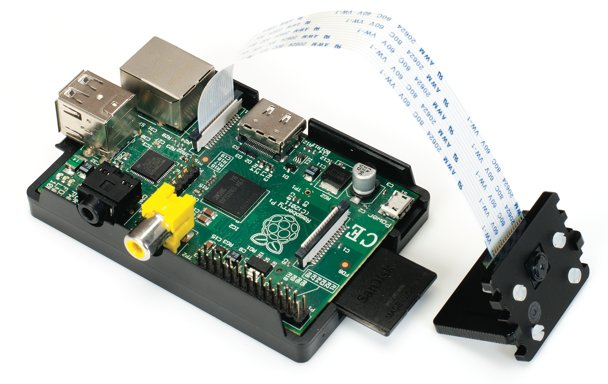
\includegraphics[scale=0.3]{6-camera}
  \caption{Raspberry Pi được lắp đặt camera chuyên dụng}\label{fig:6-camera}
\end{figure}

\textbf{Lắp đặt cảm biến khí gas:} Với các đặc tính như giá thành rẻ, độ nhạy cao và phạm vi phát hiện rộng, cảm biến khí gas MQ-2 được nhóm sử dụng để phát hiện sự xuất hiện của các khí dễ cháy như gas, cồn và khói. Cảm biến gồm có bốn chân: VCC, GND, DOUT và AOUT, hình \ref{fig:6-gas-sensor} mô tả cấu trúc bên ngoài của một cảm biến khí gas. Các chân VCC và GND lần lượt sẽ được nối vào các cổng có hiệu điện thế là 3.3V và 0V. Khi phát hiện khí gas, cổng AOUT sẽ xuất ra tính hiện tương tự (analog) còn cổng DOUT sẽ xuất ra tín hiện số (digital).

Do đặc tính các chân GPIO của Raspberry Pi chỉ nhận được tín hiệu số, nên chúng tôi chỉ sử dụng chân DOUT của cảm biến để phát hiện khí gas. Chân DOUT sẽ được đấu nối với một cổng GPIO của Raspberry PI. Bình thường, chân DOUT của cảm biến sẽ ở trạng thái High, tức có mức điện áp là 3.3V, khi phát hiện khí gas, chân DOUT sẽ ngay lập tức chuyển từ trạng thái High thành Low (0V), và trạng thái này kéo dài cho đến khi cảm biến không còn phát hiện khí gas trong không khí. Độ nhạy của cảm biến sẽ được điều chỉnh bằng tay thông qua bộ điều chỉnh màu xanh đặc bên dưới cảm biến. [3]

\begin{figure}[h]
  \centering
     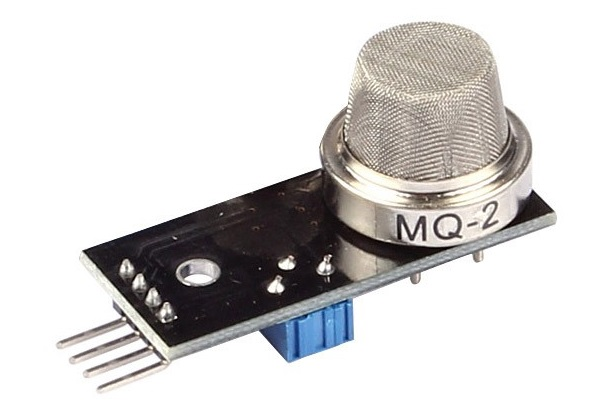
\includegraphics[scale=0.3]{6-gas-sensor}
  \caption{Module cảm biến khí gas MQ-2 [4]}\label{fig:6-gas-sensor}
\end{figure}

\textbf{Lắp đặt cảm biến ánh sáng:} Module cảm biến ánh sáng sử dụng quang trở được lựa chọn sử dụng để phát hiện thời gian hiện tại là ban ngày hay ban đêm. Khi cường độ ánh sáng tăng, điện trở của quang trở sẽ giảm và ngược lại, khi cường độ ánh sáng giảm, điện trở sẽ tăng. Giống module cảm biến khí gas MQ-2, module cảm biến ánh sáng sử dụng quang trở cũng có ba chân: VCC, GND và Signal. VCC và GND cũng sẽ được nối vào hai cổng có hiệu điện thế lần lượt là 3.3V và 0V, chân Signal được nối vào một công GPIO của Raspberry Pi. 
Khi cường độ ánh sáng thấp hơn giá trị ngưỡng, cổng Signal sẽ ở trạng thái High, tức có hiệu điện thế là 3.3V. Khi cường độ ánh sáng vượt quá giá trị ngưỡng, cổng Signal sẽ ở trạng thái Low, tức có hiệu điện thế là 0V. Giá trị ngưỡng được điều chỉnh bằng  tay sử dụng nút vặn màu xanh nằm phía dưới cảm biến. Hình \ref{fig:6-light-sensor} mô tả một con Raspberry Pi đã được kết nối với module cảm biến ánh sáng quang trở. [5][6]

\begin{figure}[h]
  \centering
     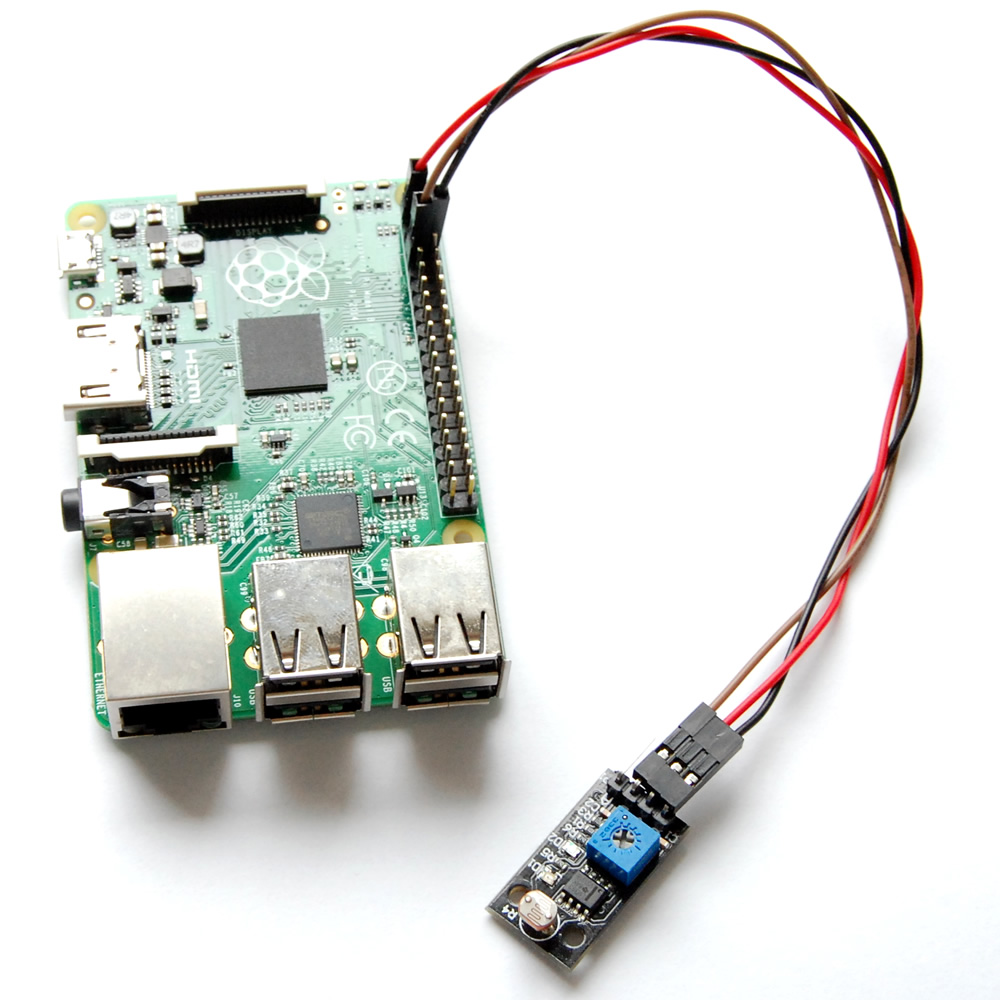
\includegraphics[scale=0.2]{6-light-sensor}
  \caption{Module cảm biến ánh sáng quang trở được gán vào Raspberry Pi [6]}\label{fig:6-light-sensor}
\end{figure}

\textbf{Lắp đặt cảm biến chuyển động:} Chức năng chống trộm cũng là một chức năng không thể thiếu của một ngôi nhà thông minh. Nhóm sử dụng module cảm biến chuyển động PIR (Passive InfraRed) để nhận biết có người hay có trộm vừa đi ngang qua. Nguyên lý hoạt động của cảm biến là dựa vào bức xạ nhiệt mà con người phát ra. Mỗi người trong chúng ta đều có thân nhiệt lúc bình thường khoảng 37 độ C và đều phát ra các bức xạ nhiệt. Khi một người đi qua, các tia bức xạ nhiệt phát ra từ người đó sẽ kích hoạt cảm biến. Hình \ref{fig:6-pir-sensor} mô tả cấu trúc bên ngoài cảm biến chuyển động PIR. [7]

\begin{figure}[h]
  \centering
     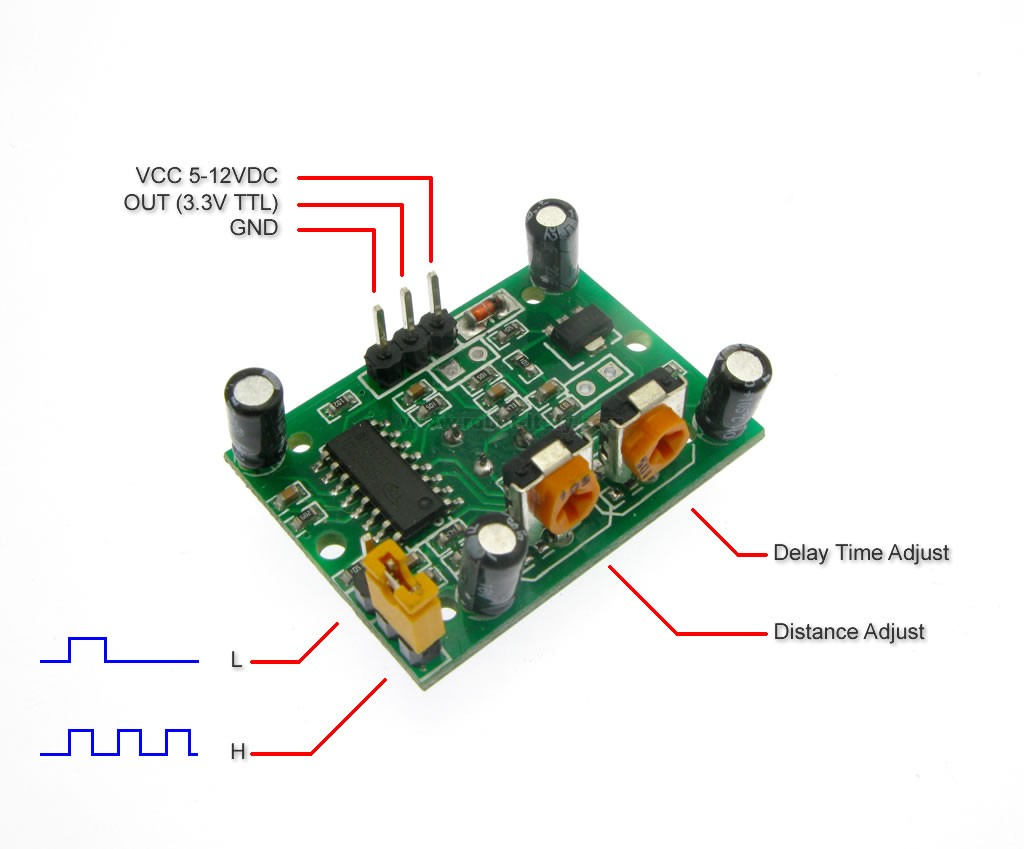
\includegraphics[scale=0.2]{6-pir-sensor}
  \caption{Cảm biến chuyển động PIR}\label{fig:6-pir-sensor}
\end{figure}

Cảm biến có ba chân: VCC, GND và OUT. Cổng VCC và GND sẽ lần lượt nối vào các cổng có hiệu điện thế lần lượt là 5V và 0V trên Raspberry Pi. Cổng OUT sẽ được nối vào một chân GPIO để ứng dụng trên Raspberry Pi có thể lấy dữ liệu từ cảm biến. Bình thường, khi không có người đi ngang qua, cổng OUT sẽ có trạng thái là Low, khi phát hiện người, trạng thái của cổng OUT là High. Khoảng cách phát hiện người và độ trễ của cảm biến có thể được điều chỉnh bằng tay qua hai bộ điều chỉnh màu cam đặt ở một cạnh của cảm biến.

\textbf{Lắp đặt cảm biến nhiệt độ:} Nhóm sử dụng cảm biến nhiệt độ DS18B20 để lấy giữ liệu về nhiệt độ trong hệ thống nhà thông minh. Cách lắp đặt cảm biến nhiệt độ này có chút phức tạp hơn so với các cảm biến khác. Cảm biến cũng gồm có ba chân: VCC, GND và OUT. Giống như các cảm biến khác, cổng VCC và GND cũng được lần lượt gắn vào các cổng có hiệu điện thế lần lượt là 3.3V và 0V. Tuy nhiên, khác với các cảm biến khác, cổng OUT của cảm biến nhiệt độ DS18B20 phải được gắn vào GPIO số 4 nằm ở vị trí số 7 trên Raspberry Pi. Bên cạnh đó, phải có một điện trở 4.7 ôm nối giữa VCC và OUT. Đầu màu vàng của cảm biến điện trở sẽ được nối vào dây VCC của cảm biến nhiệt độ. Hình \ref{fig:6-temp-sensor} mô tả cách lắp ghép cảm biến nhiệt độ DS18B20 vào Raspberry Pi.

\begin{figure}[h]
  \centering
     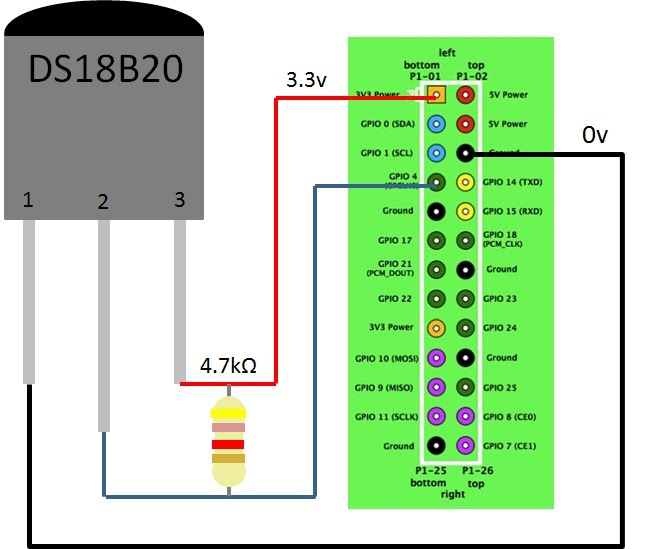
\includegraphics[scale=0.3]{6-temp-sensor}
  \caption{Cách mắc dây cho cảm biến nhiệt độ DS18B20 [11]}\label{fig:6-temp-sensor}
\end{figure}

Do cảm biến DS18B20 sử dụng cơ chế truyền tín hiệu 1-Wire nên cho phép người sử dụng có thể kết nhiều cảm biến vào cùng một chân trên Raspberry Pi. Cách kết nối cũng vô cùng đơn giản, chỉ cần kết nối tất cả cổng OUT của tất cả cảm biến vào cùng chân GPIO số 4 của Raspberry Pi. [9]

%------------------------------Hiện thực module----------------------------%
\subsection{Hiện thực module}

\begin{figure}[h]
  \centering
     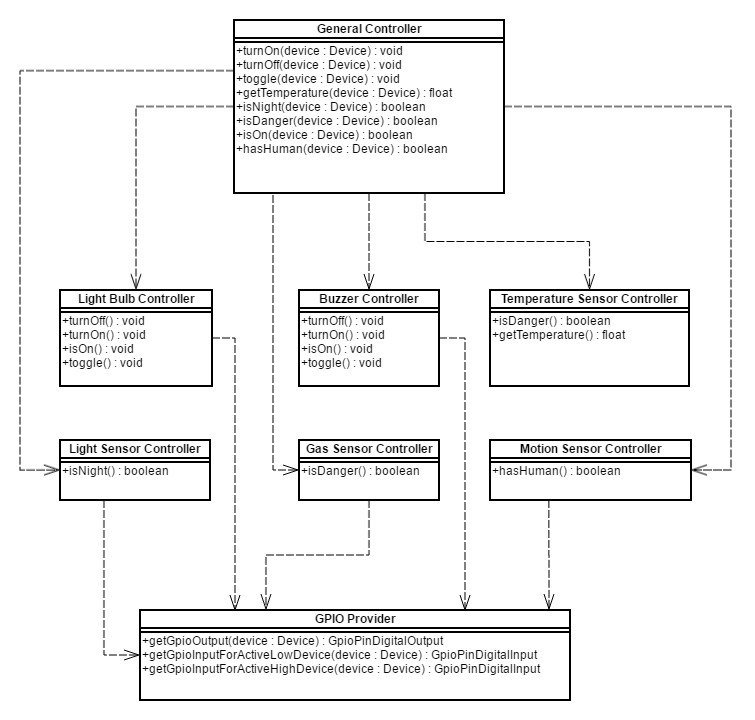
\includegraphics[scale=0.5]{6-module-dieu-khien-class-diagram}
  \caption{Sơ đồ lớp (class diagram) của module điều khiển thiết bị}\label{fig:6-module-dieu-khien-class-diagram}
\end{figure}

\textbf{Bộ điều khiển chung (GPIO Controller):} Như đã trình bày, bộ điều khiển chung sẽ nhận tất cả yêu cầu từ server. Bộ điều khiển chung cung cấp tất cả các phương thức mà server cần để lấy dữ liệu từ cảm biến cũng như điều khiển các thiết bị điện. Để sử dụng một hàm, server cần truyền vào một thực thể device. Thực thể device sẽ cung cấp tất cả các thông tin mà bộ điều khiển chung cần để thực hiện đúng hành động vào đúng thiết bị mà server cần như loại thiết bị, số thứ tự cổng GPIO… Bộ điều khiển chung sẽ dựa vào thông tin loại thiết bị và quyết định nên sử dụng bộ điều khiển thiết bị nào phù hợp. Ví dụ, server gửi yêu cầu tắt một thiết bị, trong yêu cầu của server sẽ chứa thông tin loại thiết bị mà server muốn tắt (đèn, còi,…) kèm theo số thứ tự của cổng GPIO đang điều khiển thiết bị đó. Nếu loại thiết bị là đèn, bộ điều khiển chung sử dụng bộ điều khiển đèn (Light bulb controller) để thực hiện phương thức tắt.

\textbf{Bộ cung cấp GPIO (GPIO Provider):} Trong thư viện Pi4J, để sử dụng một cổng GPIO, bước đầu tiên là khai báo cổng cần sử dụng. Bộ cung cấp GPIO có nhiệm vụ hỗ trợ các bộ điều khiển thiết bị thực hiện thao tác khai báo một cổng GPIO. Tùy thuộc vào mục đích mà một cổng GPIO có thể được khai báo là cổng nhập (input pin) hay cổng xuất (output pin). Cổng nhập (input pin) được các bộ điều khiển cảm biến sử dụng để lấy dữ liệu từ các cổng GPIO. Cổng xuất (output pin) được bộ điều khiển đèn và còi sử dụng để điều khiển việc bật hoặc tắt. Cú pháp khai báo một cổng GPIO được trình bày ở đoạn code sau:

…..

Để tránh những sự thay đổi về phần cứng sẽ ảnh hưởng đến phần mềm sử dụng các chân GPIO của Raspberry Pi, Pi4J sử dụng bộ quy tắc đánh số riêng cho những cổng GPIO. Vì thế, bộ cung cấp GPIO còn giữ vai trò chuyển đổi số thứ tự một cổng GPIO trên Raspberry Pi về số thứ tự hợp lệ trên Pi4J. Hình … mô tả cách đánh số của thư viện Pi4J trên Raspberry Pi 3 Model B. Ví dụ, cổng GPIO ở vị trí 11 trên Raspberry Pi khi chuyển đổi sang cách đánh số của thư viện Pi4J sẽ có số thứ tự là GPIO 0.

\begin{figure}[h]
  \centering
     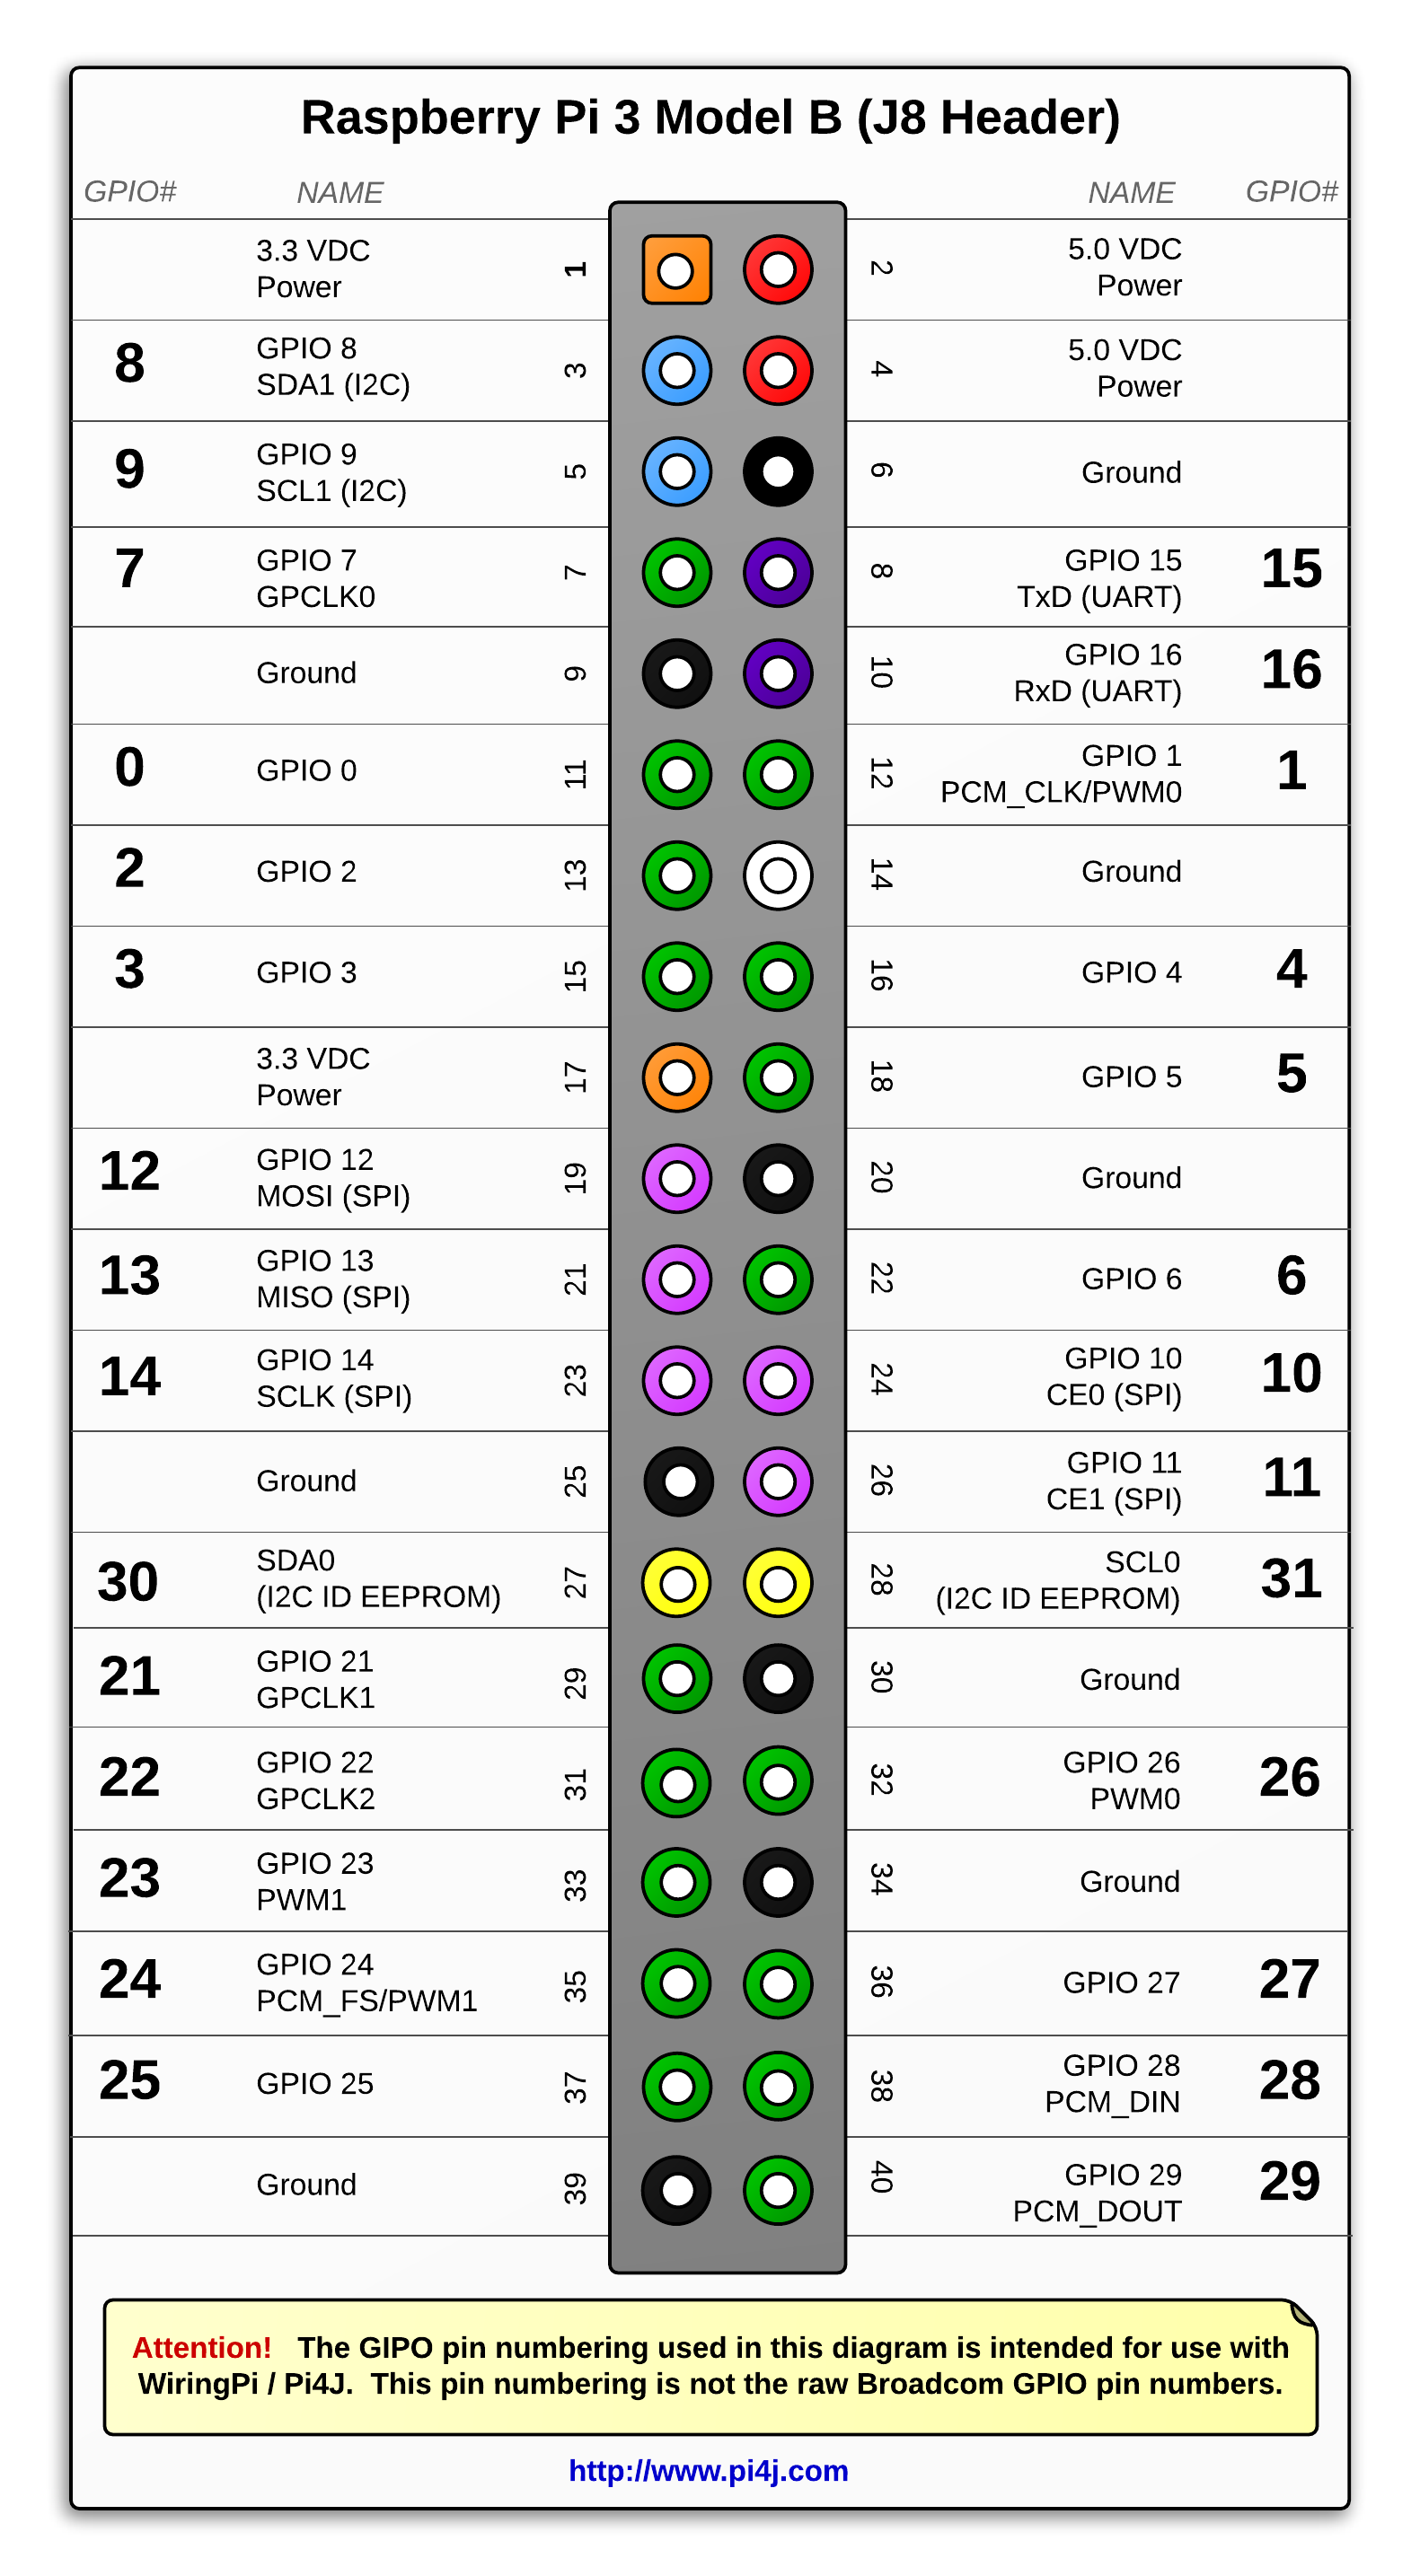
\includegraphics[width=7cm]{4-pi4j-danh-so}
  \caption{Quy tắc đánh số của Pi4J cho Raspberry Pi 3 Model B}\label{fig:4-pi4j-danh-so}
\end{figure}

\textbf{Bộ điều khiển đèn và còi:} Hai bộ điều khiển này được sử dụng bởi bộ điều khiển chung khi server có các yêu cầu liên quan đến đèn và còi. Sau khi nhận yêu cầu từ server, bộ điều khiển chung sẽ truyền thông tin về cổng GPIO đến đúng bộ điều khiển. Khi nhận thông tin về số thứ tự cổng GPIO, bộ điều khiển đèn hoặc còi sẽ sử dụng bộ cung cấp GPIO để khởi tạo đúng loại cổng, input pin hay output pin.
Như đã trình bày, mỗi cổng GPIO sẽ có hai trạng thái là Low hoặc High. Bộ điều khiển đèn và còi sẽ điều khiển các thiết bị bằng cách thay đổi trạng thái của chân GPIO đang điều khiển thiết bị đó. Tùy loại thiết bị mà trạng thái High hoặc Low sẽ tương ứng với việc bật hay tắt và ngược lại. Ví dụ, nếu loại đèn được sử dụng là tích cực mức thấp, khi chân GPIO ở trạng thái Low thì đèn sẽ sáng và ngược lại. Loại đèn và còi mà nhóm đang sử dụng để thuộc loại tích cực mức thấp. Cú pháp thay đổi trạng thái một cổng GPIO khi sử dụng thư viện Pi4J thể hiện như sau:

…

\textbf{Bộ điều khiển cảm biến ánh sáng, chuyển động và khí gas:}

%-------------------------------Phát triển ứng dụng di động-------------------%
\newpage
\section{Phát triển ứng dụng di động}
\subsection{Hướng phát triển ứng dụng di động}
Hiện nay có 2 xu hướng phát triển ứng dụng di động chính là: Phát triển ứng dụng di động thuần túy (Native Mobile Application Development) và Phát triển ứng dụng di động lại (Hybrid Mobile Application Development).

\textbf{Phát triển ứng dụng di động thuần túy (Native Mobile Application Development):} phát triển ứng dụng di động thuần túy là phát triển một ứng dụng đặc biệt chỉ chạy trên một hệ điều hành nhất định thuộc một thiết bị nhất định, với ngôn ngữ phát triển cụ thể (như Objective-C hoặc Swift cho hệ điều hành iOS hoặc Java cho hệ điều hành Android), và thường phải thông qua điều chỉnh để có thể chạy được trên nhiều thiết bị khác nhau [4].

Vì ứng dụng được phát triển hoàn toàn trong môi trường dành riêng cho một hệ điều hành nhất định, với những đặc tính kỹ thuật và giao diện đặc trưng của hệ điều hành đó, nên không chỉ có lợi thế về hiệu xuất, ứng dụng di động thuần túy còn có lợi thế trong trải nghiệm người dùng. Lợi thế trong trải nghiệm người dùng ở đây là ứng dụng có được sự đồng nhất về mặt giao diện và cảm nhận với nhiều ứng dụng thuần túy khác trên thiết bị. Người dùng có thể dễ dàng nắm bắt cách thức sử dụng cũng như tương tác với ứng dụng một cách nhanh chóng hơn. Ngoài ra, những ứng dụng di động thuần túy có lợi thế không nhỏ trong việc có khả năng truy cập và sử dụng một cách dễ dàng những tính năng đặc thù của thiết bị (GPS, sổ địa chỉ, camera, bộ phận cảm ứng…) [3].

\textbf{Phát triển ứng dụng di động lai (Hybrid Mobile Application Development):} phát triển ứng dụng di động lai là phát triển ứng dụng dựa trên nền tảng Web, sử dụng công nghệ phổ biến là HTML5 và JavaScript, được đóng gói lại trong một thành phần thuần túy (native container). Thành phần này thực hiện việc tải phần lớn thông tin lên giao diện khi người dùng truy cập qua từng chức năng của ứng dụng [3].

\begin{table}[!htbp]
\centering
\caption{So sánh điểm mạnh, điểm yếu của Phát triển ứng dụng di động thuần túy và Phát triển ứng dụng di động lai [4]}\label{tab:compare-native-and-hybrid}
\begin{tabular}{ |p{2cm}|p{6cm}|p{6cm}| }
\hline
	So sánh & 
	\begin{tabular}[t]{p{5.5cm}}
	Phát triển ứng dụng di động thuần túy
	\end{tabular} &	
	\begin{tabular}[t]{p{5.5cm}}
	Phát triển ứng dụng di động lai
	\end{tabular}\\
\hline
	Điểm mạnh &
	\begin{tabular}[t]{p{5.5cm}}
	- Về mặt hiệu năng, trong hầu hết trường hợp, ứng dụng di động thuần túy chạy nhanh hơn ứng dụng lai nhưng sự chênh lệch không quá lớn và thường khó nhận biết bởi người dùng.\\
	- Về tính năng, ứng dụng di động thuần túy có thể dễ dàng truy cập tới phần cứng của thiết bị (camera, thiết bị thu âm…) cũng như truy cập tới các chức năng đặc quyền như sao chép, tạo, ghi dữ liệu trên bộ nhớ, thông tin danh bạ, cuộc gọi, tin nhắn… so với ứng dụng di động lại còn nhiều hạn chế về việc tận dụng toàn bộ sức mạnh của thiết bị.\\
	- Khi không có kết nối Internet, ứng dụng di động thuần túy có thể sử dụng những dữ liệu đã lưu trữ tạm (cache) trước đó trong khi ứng dụng lai đa phần đều cần phải có kết nối Internet để truy cập dữ liệu.
	\end{tabular} &
	\begin{tabular}[t]{p{5.5cm}}
	- Người phát triển không bị hạn chế vào một hệ điều hành nhất định, có thể phát triển chỉ một ứng dụng nhưng chạy được trên nhiều hệ điều hành khác nhau.\\
	- Chi phí cho việc phát triển, bảo trì và nâng cấp ứng dụng sẽ được giảm thiểu đáng kể vì chỉ có một phiên bản duy nhất.\\
	- Ngôn ngữ lập trình cho ứng dụng di động lai là HTML và JavaScript rất phổ dụng, đa số người phát triển đều biết.
	\end{tabular}\\
\hline
	Điểm yếu &
	\begin{tabular}[t]{p{5.5cm}}
	- Ứng dụng di động thuần túy không thể chạy trên nhiều hệ điều hành khác nhau, nói cách khác, một ứng dụng di động thuần túy chỉ chạy được trên một hệ điều hành nhất định.\\
	- Khi muốn phát triển đa nền tảng, phát triển ứng dụng di động thuần túy sẽ có chi phí phát triển ca vì đòi hỏi khả năng thành thạo nhiều ngôn ngữ của người phát triển.\\
	- Sự đa dạng các phiên bản hệ điều hành gây cản trở tính tương thích của các ứng dụng di động thuần túy.
	\end{tabular} &
	\begin{tabular}[t]{p{5.5cm}}
	- Về mặt hiệu năng, đa phần các ứng dụng di động lai không chạy nhanh bằng các ứng dụng di động thuần túy.\\
	- Ứng dụng di động lai thường không tận dụng được tối đa các tính năng phần cứng, sức mạnh của thiết bị.\\
	- Một số chợ ứng dụng sẽ không chấp nhận ứng dụng lai được đăng lên nếu như không hoạt động đủ trơn tru.
	\end{tabular}\\
\hline
\end{tabular}
\end{table}

Để có thể hỗ trợ được nhiều nền tảng di động một cách dễ dàng và tiết kiệm thời gian, đồng thời vì kiến trúc ứng dụng không quá phức tạp và không đòi hỏi nhiều tới những tính năng phần cứng đặc thù của thiết bị, chúng tôi quyết định sẽ phát triển ứng dụng di động theo hướng \textbf{Phát triển ứng dụng di động lai (Hybrid Mobile Application Development)}.

\subsection{Các công nghệ sử dụng}
Theo hướng phát triển ứng dụng di động lai, ứng dụng cần được xây dựng trên nền tảng Web. Giao diện Web của ứng dụng sẽ được thiết kế tập trung vào việc hỗ trợ cho thiết bị di động. Sau đó, ứng dụng sẽ được chuyển tiếp từ nền tảng Web sang các nền tảng di động thông qua các công nghệ hỗ trợ.

Các công nghệ chính được sử dụng để phát triển ứng dụng:
\begin{itemize}[topsep=1mm,itemsep=-0.5mm]
\item AngularJS – Công nghệ được sử dụng để phát triển ứng dụng trên nền tảng Web
\item Apache Cordova – Công nghệ được sử dụng để chuyển tiếp ứng dụng từ nền tảng Web sang các nền tảng di động khác nhau
\vspace{1mm}
\end{itemize}

\textbf{AngularJS:} AngularJS là một framework mạnh mẽ mã nguồn mở có cấu trúc hỗ trợ phát triển ứng dụng Web động. Framework này cho phép sử dụng HTML như là một ngôn ngữ mẫu, đồng thời cho phép mở rộng các cú pháp HTML để diễn đạt các thành phần của ứng dụng một cách rõ ràng và ngắn gọn. Hai tính năng chính của AngularJS là Liên kết dữ liệu (Data Binding) và Tiêm nhiễm phụ thuộc (Dependency Injection) giúp loại bỏ phần lớn mã code mà người phát triển ứng dụng thường phải viết.

Các đặc tính của AngularJS:
\begin{itemize}[topsep=1mm,itemsep=-0.5mm]
\item AngularJS hỗ trợ người phát triển viết ứng dụng theo mô hình MVC (Model View Controller)
\item Các ứng dụng AngularJS có khả năng tương thích với hầu hết các trình duyệt web với nhiều phiên bản trên các nền tảng khác nhau
\item AngularJS là framework mã nguồn mở, hoàn toàn miễn phí và được sử dụng rộng rãi bởi hàng ngàn lập trình viên trên thế giới
\vspace{1mm}
\end{itemize}

Các tính năng và thành phần cốt lõi của AngularJS:

\begin{itemize}[topsep=1mm,itemsep=-0.5mm]
\item \textbf{Khung nhìn (View):} là những gì mà người dùng nhìn thấy được.
\item \textbf{Mô hình (Model):} dữ liệu nằm trên View mà có thể tương tác.
\item \textbf{Liên kết dữ liệu (Data Binding):} đồng bộ dữ liệu giữa 2 thành phần model và view.
\item \textbf{Chỉ thị (Directive):} mở rộng các thẻ HTML với các đặc tính và yếu tố tự tạo.
\item \textbf{Bộ quản lý (Controller):} xử lý các thao tác nghiệp vụ bên dưới các Khung nhìn.
\item \textbf{Biểu thức (Expression):} truy cập các biến và hàm từ Phạm vi.
\item \textbf{Phạm vi (Scope):} phạm vi nơi các Mô hình được lưu trữ để các Bộ quản lý, Chỉ thị và Biểu thức có thể truy cập.
\item \textbf{Dịch vụ (Service):} những thao tác nghiệp vụ có thể sử dụng lại độc lập với các Khung nhìn.
\item \textbf{Tiêm nhiễm phụ thuộc (Dependency Injection):} tạo và liên kết các đối tượng và hàm.
\vspace{1mm}
\end{itemize}

Với các tính năng hỗ trợ phù hợp với kiến trúc của ứng dụng, cộng với sự phổ biến và được sử dụng rộng rãi của AngularJS. Nhóm chúng tôi quyết định sử dụng công nghệ này để phát triển ứng dụng trên nền tảng Web.

\textbf{Apache Cordova:} Apache Cordova là một framework mã nguồn mở hỗ trợ phát triển ứng dụng di động trên nền tảng Web. Framework này cho phép sử dụng những kĩ thuật Web chuẩn như HTML5, CSS3 và JavaScript để phát triển. Ứng dụng Web được xây dựng sẽ được chuyển tiếp thành ứng dụng trên các nền tảng di động gốc và dựa trên các API ràng buộc chuẩn để truy cập tới các chức năng của từng thiết bị như cảm biến, dữ liệu, tình trạng mạng…

Apache Cordova thường được sử dụng khi:

\begin{itemize}[topsep=1mm,itemsep=-0.5mm]
\item Người phát triển ứng dụng di động muốn mở rộng ứng dụng từ một nền tảng sang nhiều nền tảng khác, mà không cần phải phát triển lại toàn bộ ứng dụng theo từng ngôn ngữ lập trình và công cụ riêng của từng nền tảng.
\item Người phát triển ứng dụng Web muốn đưa ứng dụng lên nhiều nền tảng cũng như nhiều cửa hàng ứng dụng khác nhau.
\item Người phát triển ứng dụng di động muốn pha trộn nhiều thành phần thuộc nền tảng di động gốc và các thành phần này có thể  truy cập tới các API cấp thiết bị.
\vspace{1mm}
\end{itemize}

Các nền tảng hỗ trợ:

\begin{figure}[h]
  \centering
     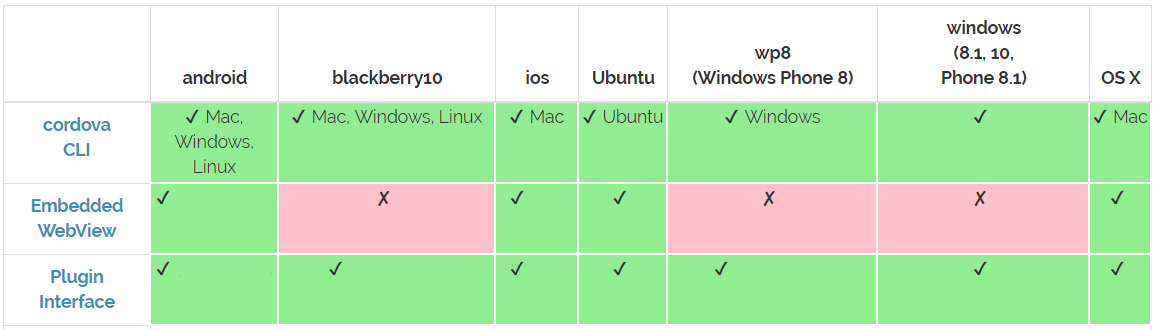
\includegraphics[width=15cm]{6-cordova-platforms}
  \caption{Bảng các nền tảng Apache Cordova hỗ trợ}\label{fig:6-cordova-platforms}
\end{figure}

Với tính đơn giản dễ sử dụng, đồng thời có khả năng hỗ trợ nhiều nền tảng di động khác nhau, đặc biệt là 3 nền tảng di động chính được sử dụng rộng rãi hiện nay là Android, iOS và Windows Phone, nhóm chúng tôi quyết định sử dụng công nghệ Apache Cordova để chuyển tiếp ứng dụng từ nền tảng Web sang các nền tảng di động khác nhau.

\subsection{Hiện thực ứng dụng di động}
Cấu trúc của ứng dụng di động bao gồm 3 mảng: Các thành phần chính (components), các thành phần đóng góp (shared), và Dịch vụ chính (Main Service). Các thành phần chính phản ánh kiến trúc của ứng dụng di động ở Phần 5, với mỗi thành phần chính tương ứng với từng Giao diện chính của ứng dụng. Trong khi đó, các thành phần đóng góp là các thành phần chung được sử dụng lại nhiều lần giữa các thành phần chính khác nhau hoặc trong cùng một thành phần chính. Dịch vụ chính đảm nhiệm vai trò gọi các API Web Service từ phía Server để lấy dữ liệu, đồng thời thực hiện việc cập nhật trạng thái và đồng bộ liên kết giữa các thành phần chính và các thành phần đóng góp với nhau.

\textbf{Các thành phần đóng góp (shared):} Các thành phần đóng góp trong ứng dụng bao gồm 8 thành phần: Thanh công cụ (Navbar), Thẻ nhà (Home-panel), Thẻ kiểu thiết bị (Device-type-panel), Thẻ thiết bị (Device-panel), Thẻ kịch bản (Device-script-panel), Thẻ kịch bản khi/thì (Device-script-when-then), Thẻ kịch bản từ/đến (Device-script-from-to) và Thẻ kịch bản tự tạo (Device-script-custom). Các thành phần này thực chất là các Chỉ thị (Directive) của AngularJS, với mỗi thành phần có một giao diện với một bộ quản lý (controller) đảm nhận các xử lý nghiệp vụ riêng. Vì bản chất là Chỉ thị (Directive), mỗi thành phần đều có thể dễ dàng gắn vào nhau hoặc vào các thành phần chính như là một dạng thẻ HTML bình thường.

Thanh công cụ (Navbar):

\begin{figure}[h]
  \centering
     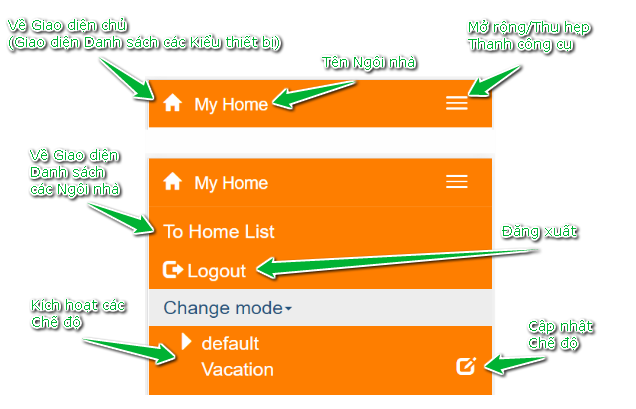
\includegraphics[width=10cm]{6-navbar}
  \caption{Thanh công cụ (Navbar)}\label{fig:6-navbar}
\end{figure}

Thanh công cụ (Navbar) là thành phần đóng góp cho phép người dùng thực hiện một số các thao tác cơ bản của ứng dụng một cách nhanh chóng, được sử dụng ở các thành phần chính là: Thành phần Danh sách các Ngôi nhà, Thành phần Danh sách các Kiểu thiết bị và Thành phần Danh sách các thiết bị. Thanh công cụ có nhiều chức năng khác nhau tùy thuộc vào thành phần chính mà nó được sử dụng. Các chức năng của thanh công cụ:

\begin{itemize}[topsep=1mm,itemsep=-0.5mm]
\item Thể hiện tên của Ngôi nhà hiện tại đang truy cập.
\item Cho phép người dùng quay lại Giao diện Danh sách các Kiểu thiết bị.
\item Cho phép người dùng đăng xuất.
\item Cho phép người dùng kích hoạt các Chế độ
\item Cho phép người dùng xem, cập nhật chỉnh sửa thông tin hoặc xóa các Chế độ.
\vspace{1mm}
\end{itemize}

Thẻ nhà (Home-panel):

\begin{figure}[h]
  \centering
     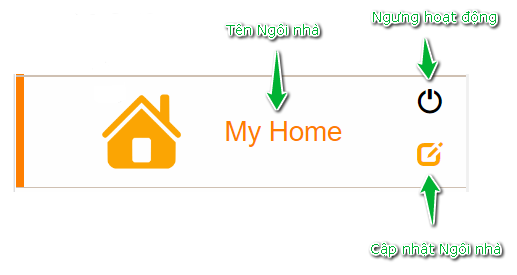
\includegraphics[width=12cm]{6-home-panel}
  \caption{Thẻ nhà}\label{fig:6-home-panel}
\end{figure}

Thẻ nhà (Home-panel) là thành phần đóng góp thể hiện thông tin của một ngôi nhà được lắp đặt hệ thống, thành phần này được sử dụng nhiều lần như một danh sách trong thành phần chính Danh sách các Ngôi nhà. Các chức năng của thẻ nhà:

\begin{itemize}[topsep=1mm,itemsep=-0.5mm]
\item Thể hiện tên của ngôi nhà.
\item Cho phép người dùng ngưng hoạt động tạm thời (Disable) hoặc tái hoạt động (Enable) ngôi nhà.
\item Cho phép người dùng xem, cập nhật chỉnh sửa thông tin hoặc xóa ngôi nhà.
\item Chuyển tiếp người dùng tới thành phần chính Danh sách các Kiểu thiết bị.
\vspace{1mm}
\end{itemize}

Thẻ Kiểu thiết bị (Device-type-panel):

\begin{figure}[h]
  \centering
     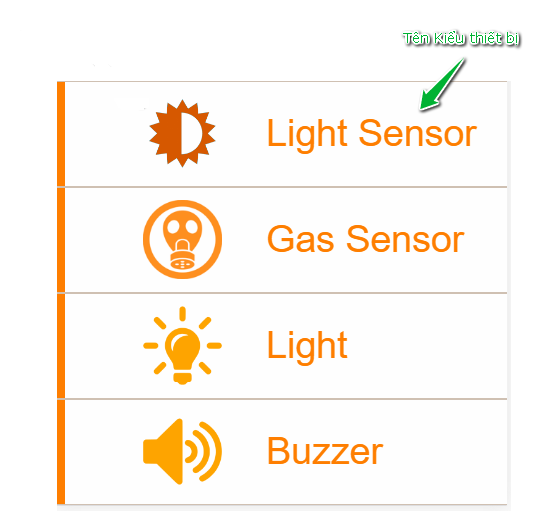
\includegraphics[width=10cm]{6-device-type-panels}
  \caption{Một số Thẻ kiểu thiết bị}\label{fig:6-device-type-panels}
\end{figure}

Thẻ Kiểu thiết bị (Device-type-panel) là thành phần đóng góp thể hiện thông tin của một kiểu thiết bị được hệ thống hỗ trợ, thành phần này được sử dụng nhiều lần như một danh sách trong thành phần chính Danh sách Các kiểu thiết bị. Ứng với mỗi kiểu thiết bị thì thẻ Kiểu thiết bị có kí hiệu thể hiện và tên khác nhau, có 6 kiểu thiết bị hỗ trợ: Cảm biến nhiệt độ (Temperature Sensor), Cảm biến chuyển động (Motion Sensor), Cảm biến ánh sánh (Light Sensor), Cảm biến khí gas (Gas Sensor), Bóng đèn (Light) và Còi hú (Buzzer). Các chức năng của Thẻ Kiểu thiết bị:

\begin{itemize}[topsep=1mm,itemsep=-0.5mm]
\item Thể hiện thông tin của Kiểu thiết bị.
\item Chuyển tiếp người dùng tới thành phần chính Danh sách các thiết bị.
\vspace{1mm}
\end{itemize}

Thẻ Thiết bị (Device-panel)

\begin{figure}[h]
  \centering
     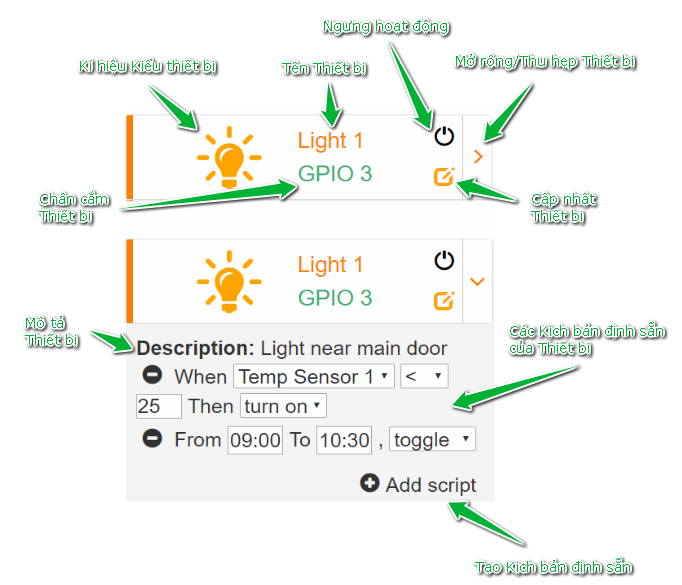
\includegraphics[width=10cm]{6-device-panel}
  \caption{Thẻ Thiết bị}\label{fig:6-device-panel}
\end{figure}

Thẻ Thiết bị (Device-panel) là thành phần đóng góp thể hiện thông tin của một thiết bị cùng với các Kịch bản định sẵn của thiết bị đó, được sử dụng nhiều lần như một danh sách trong thành phần chính Danh sách các Thiết bị. Thành phần này chứa bên trong nó một tập hợp các thành phần đóng góp Thẻ Kịch bản để hỗ trợ việc thể hiện thông tin các Kịch bản thuộc thiết bị. Các chức năng của Thẻ thiết bị:

\begin{itemize}[topsep=1mm,itemsep=-0.5mm]
\item Thể hiện kiểu, tên và chân cắm của thiết bị.
\item Cho phép người dùng ngưng hoạt động tạm thời (Disable) hoặc tái hoạt động (Enable) thiết bị.
\item Cho phép người dùng xem, cập nhật chỉnh sửa thông tin hoặc xóa thiết bị.
\item Cho phép người dùng xem thông tin các Kịch bản định sẵn của thiết bị.
\item Cho phép người dùng tạo thêm Kịch bản định sẵn cho thiết bị.
\vspace{1mm}
\end{itemize}

Thẻ Kịch bản (Device-script-panel)

Thẻ Kịch bản (Device-script-panel) chứa bên trong nó 2 thành phần đóng góp khác là Thẻ Kịch bản khi/thì (Device-script-when-then) và Thẻ Kịch bản từ/đến (Device-script-from-to). Tùy vào loại Kịch bản được truyền vào mà thành phần này sẽ quyết định lựa chọn một trong hai thành phần đóng góp bên trong nó để thể hiện.

Thẻ Kịch bản khi/thì (Device-script-when-then)

\begin{figure}[h]
  \centering
     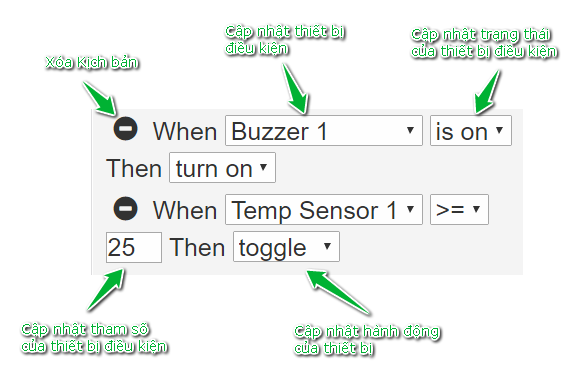
\includegraphics[width=10cm]{6-device-script-when-then}
  \caption{Một số Thẻ Kịch bản khi/thì}\label{fig:6-device-script-when-then}
\end{figure}

Thẻ Kịch bản khi/thì (Device-script-when-then) là thành phần đóng góp thể hiện thông tin của một kịch bản thuộc loại Khi/thì (When/Then), với 2 bộ phận là Điều kiện và Hành động. Bộ phận Điều kiện gồm 3 bộ phận nhỏ hơn là Thiết bị điều kiện, Trạng thái của thiết bị điều kiện và Tham số của thiết bị điều kiện. Tham số của thiết bị điều kiện có được thể hiện hay không tùy thuộc vào kiểu của thiết bị điều kiện. Các chức năng của Thẻ Kịch bản khi/thì:

\begin{itemize}[topsep=1mm,itemsep=-0.5mm]
\item Thể hiện nội dung bao gồm Điều kiện và Hành động của kịch bản thuộc loại Khi/thì.
\item Cho phép người dùng cập nhật chỉnh sửa thiết bị điều kiện.
\item Cho phép người dùng cập nhật chỉnh sửa trạng thái của thiết bị điều kiện.
\item Cho phép người dùng cập nhật chỉnh sửa tham số của thiết bị điều kiện.
\item Cho phép người dùng cập nhật chỉnh sửa hành động của thiết bị.
\item Cho phép người dùng xóa kịch bản.
\vspace{1mm}
\end{itemize}

Thẻ Kịch bản từ/đến (Device-script-from-to)

\begin{figure}[h]
  \centering
     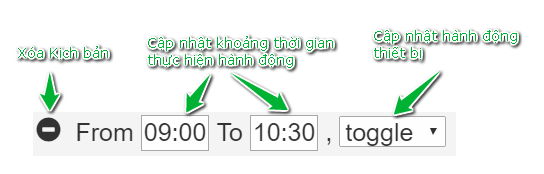
\includegraphics[width=10cm]{6-device-script-from-to}
  \caption{Thẻ Kịch bản từ/đến}\label{fig:6-device-script-from-to}
\end{figure}

Thẻ Kịch bản từ/đến (Device-script-from-to) là thành phần đóng góp thể hiện thông tin của một kịch bản thuộc loại Từ/đến (From/To), với 2 bộ phận là Khoảng thời gian hành động được thực hiện và Hành động. Các chức năng của thể Kịch bản từ/đến:

\begin{itemize}[topsep=1mm,itemsep=-0.5mm]
\item Thể hiện nội dung bao gồm Khoảng thời gian hành động được thực hiện và Hành động của kịch bản thuộc loại từ/đến.
\item Cho phép người dùng cập nhật chỉnh sửa khoảng thời gian thực hiện hành động của thiết bị.
\item Cho phép người dùng cập nhật chỉnh sửa hành động của thiết bị.
\item Cho phép người dùng xóa kịch bản.
\vspace{1mm}
\end{itemize}

\newpage
\section{Đánh giá tích hợp hệ thống}

%-------------------------------------Tổng kết----------------------------------%
\chapter{Tổng kết}

%-------------------------------------Tài liệu tham khảo------------------------%
\newpage
\bibliographystyle{abbrv}
\bibliography{references}

%--------------------------------------Phụ lục--------------------------------%
\chapter*{Phụ lục} 
\addcontentsline{toc}{chapter}{Phụ lục}

\end{document}
